\newpage

% ##############################################

\noindent Naming

\noindent  Figure - fig. 1 \\
lable: \\
equation - eq:NAME \\
table - table:NAME \\
algorithm - agl:NAME \\
figure - fig:NAME \\

% ##############################################

This is cite example. \cite{IEEEexample:bluebookbook}

This is reference. \cref{sec:conclusion,sec:designanddevelopment} or \ref{sec:introduction}
\newline
Eqution - \cref{eq:name} \\
Table - \cref{tab1e:name} \\
Algorithm - \cref{alg:interactive_sinhala_qas} \\
Figure - \cref{fig:name1} \\
\newline

% ##############################################

\begin{itemize}
    \item Use either SI (MKS) or CGS as primary units. (SI units are encouraged.) English units may be used as secondary units (in parentheses). An exception would be the use of English units as identifiers in trade, such as ``3.5-inch disk drive''.
    \item Avoid combining SI and CGS units, such as current in amperes and magnetic field in oersteds. This often leads to confusion because equations do not balance dimensionally. If you must use mixed units, clearly state the units for each quantity that you use in an equation.
    \item Do not mix complete spellings and abbreviations of units: ``Wb/m\textsuperscript{2}'' or ``webers per square meter'', not ``webers/m\textsuperscript{2}''. Spell out units when they appear in text: ``. . . a few henries'', not ``. . . a few H''.
    \item Use a zero before decimal points: ``0.25'', not ``.25''. Use ``cm\textsuperscript{3}'', not ``cc''.)
\end{itemize}

% ##############################################

\begin{equation}
    a+b=\gamma\label{eq:name}
\end{equation}

% ##############################################

Use https://www.latex-tables.com/ to create table

\begin{table}[htbp]
    \caption{Table Type Styles}
    \begin{center}
        \begin{tabular}{|c|c|c|c|}
            \hline
            \textbf{Table} & \multicolumn{3}{|c|}{\textbf{Table Column Head}}                                                         \\
            \cline{2-4}
            \textbf{Head}  & \textbf{\textit{Table column subhead}}           & \textbf{\textit{Subhead}} & \textbf{\textit{Subhead}} \\
            \hline
            copy           & More table copy$^{\mathrm{a}}$                   &                           &                           \\
            \hline
            \multicolumn{4}{l}{$^{\mathrm{a}}$Sample of a Table footnote.}
        \end{tabular}
        \label{tab1e:name}
    \end{center}
\end{table}

\begin{table}[htbp]
    \centering
    \caption{Model performance comparison}
    \begin{tabular}{lcc}
        \toprule
        \textbf{Model} & \textbf{Accuracy (\%)} & \textbf{F1-score} \\
        \midrule
        CNN            & 92.1                   & 0.88              \\
        Transformer    & 95.3                   & 0.91              \\
        Ours           & \textbf{97.6}          & \textbf{0.94}     \\
        \bottomrule
    \end{tabular}
    \label{tab:results}
\end{table}

\begin{table}[htbp]
    \centering
    \caption{Dataset statistics}
    \begin{tabular}{lcc}
        \toprule
        \textbf{Category}         & \textbf{Class} & \textbf{Samples} \\
        \midrule
        \multirow{2}{*}{Animals}  & Cats           & 500              \\
                                  & Dogs           & 600              \\
        \multirow{2}{*}{Vehicles} & Cars           & 700              \\
                                  & Trucks         & 400              \\
        \bottomrule
    \end{tabular}
    \label{tab:dataset}
\end{table}


% ##############################################

\begin{algorithm}
    \caption{Interactive Sinhala Question and Answer System}
    \label{alg:interactive_sinhala_qas}
    \begin{algorithmic}[1]
        \Require Sinhala question as voice input, object image
        \Ensure Identified objects in the image with labels
        \Repeat
        \Comment{Loop indefinitely until a break condition}
        \State $image \gets \text{CaptureImage}()$
        \State $detectedObjects \gets \text{YOLODetection}(image)$
        \State $context \gets \emptyset$ \Comment{Initialize empty context list}
        % \Statex
        \ForAll{$SinhalaLabel \in detectedObjects$}
        \If{$\text{ExistsInMongoDB}(SinhalaLabel)$}
        \State $info \gets \text{RetrieveSinhalaInfo}(label)$
        \State $context \gets context \cup \{info\}$
        \EndIf
        \EndFor
        % \Statex
        \State $voiceInput \gets \text{GetUserVoiceInput}()$
        \State $question \gets \text{GCPSpeechToTextAPI}(voiceInput)$
        % \Statex
        \If{$context \neq \emptyset$}
        \State $model \gets \text{LoadSinhalaBERT}()$
        \State $answer \gets \text{GenerateSinhalaAnswer}(model,$
            \Statex \hspace{2.8em} $question, context)$
        \Else
        \State $answer \gets \text{"No context found"}$
        \EndIf
        % \Statex
        \State $speech \gets \text{GCPTextToSpeechAPI}(answer)$
        \State $\text{OutputSpeechToSpeaker}(speech)$
        % \Statex
        \If{$\text{TerminationRequested}()$}
        \State \textbf{break}
        \EndIf

        \Until{termination condition is met}
    \end{algorithmic}
\end{algorithm}


% ##############################################

% \begin{figure}[htbp]
%     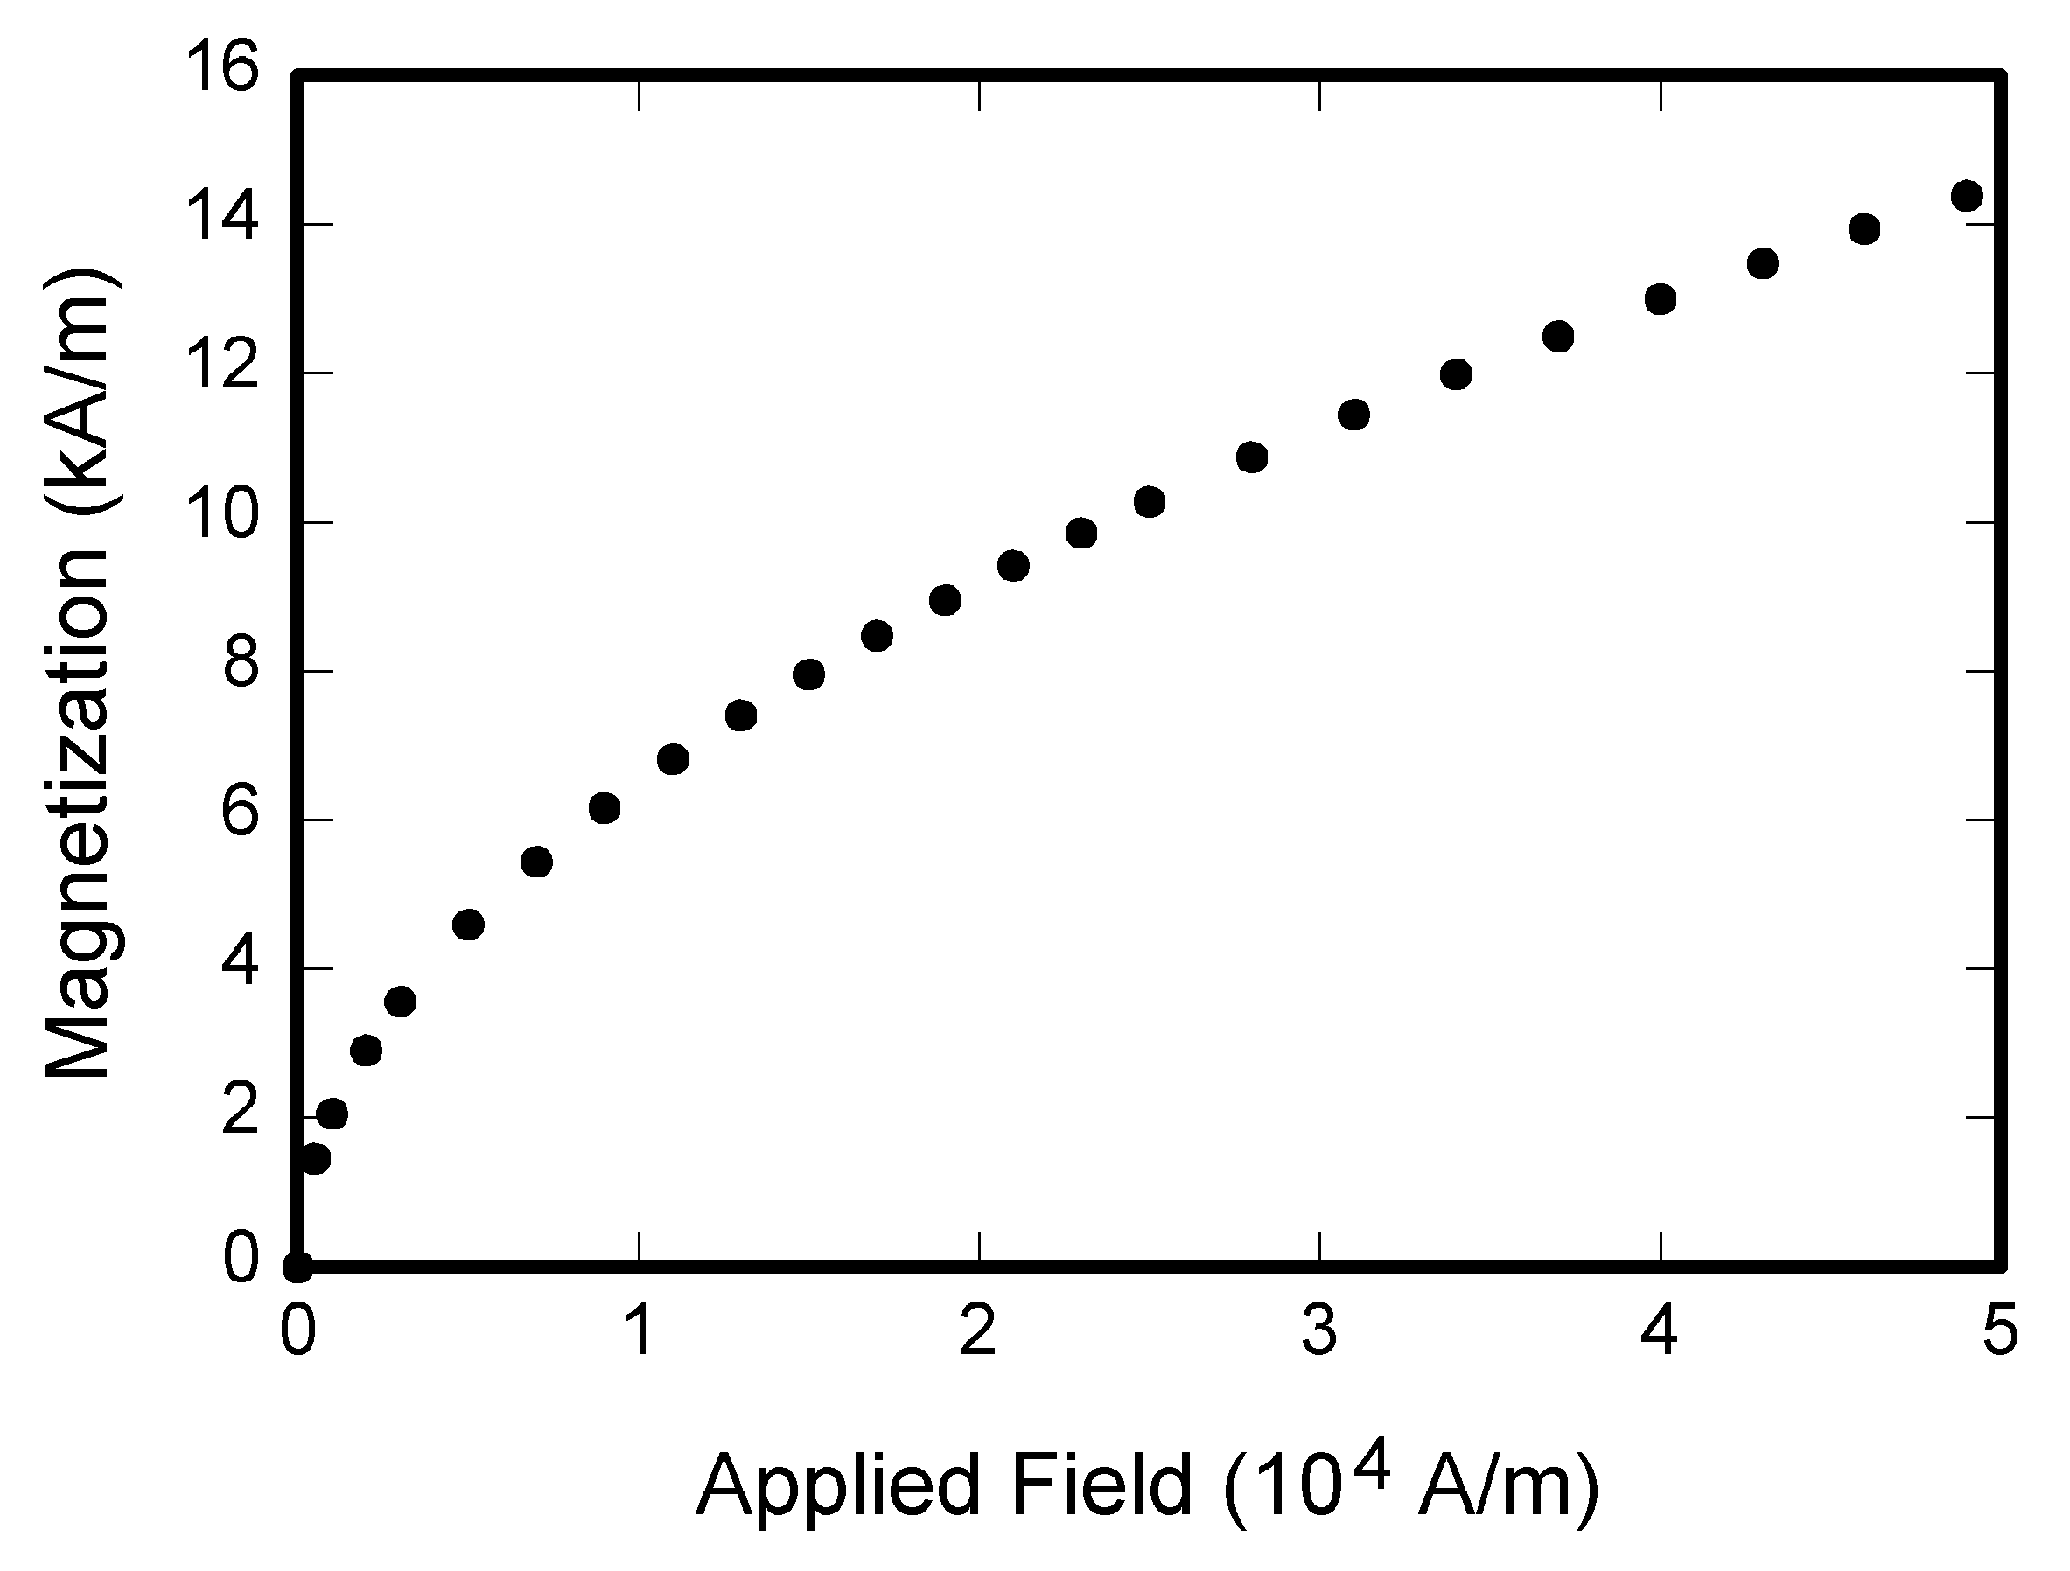
\includegraphics[width=3.5in]{Photos/fig1.png}
%     \caption{Example of a figure caption. - ONE Column}
%     \label{fig:name1}
% \end{figure}

% \begin{figure*}[htbp]
%     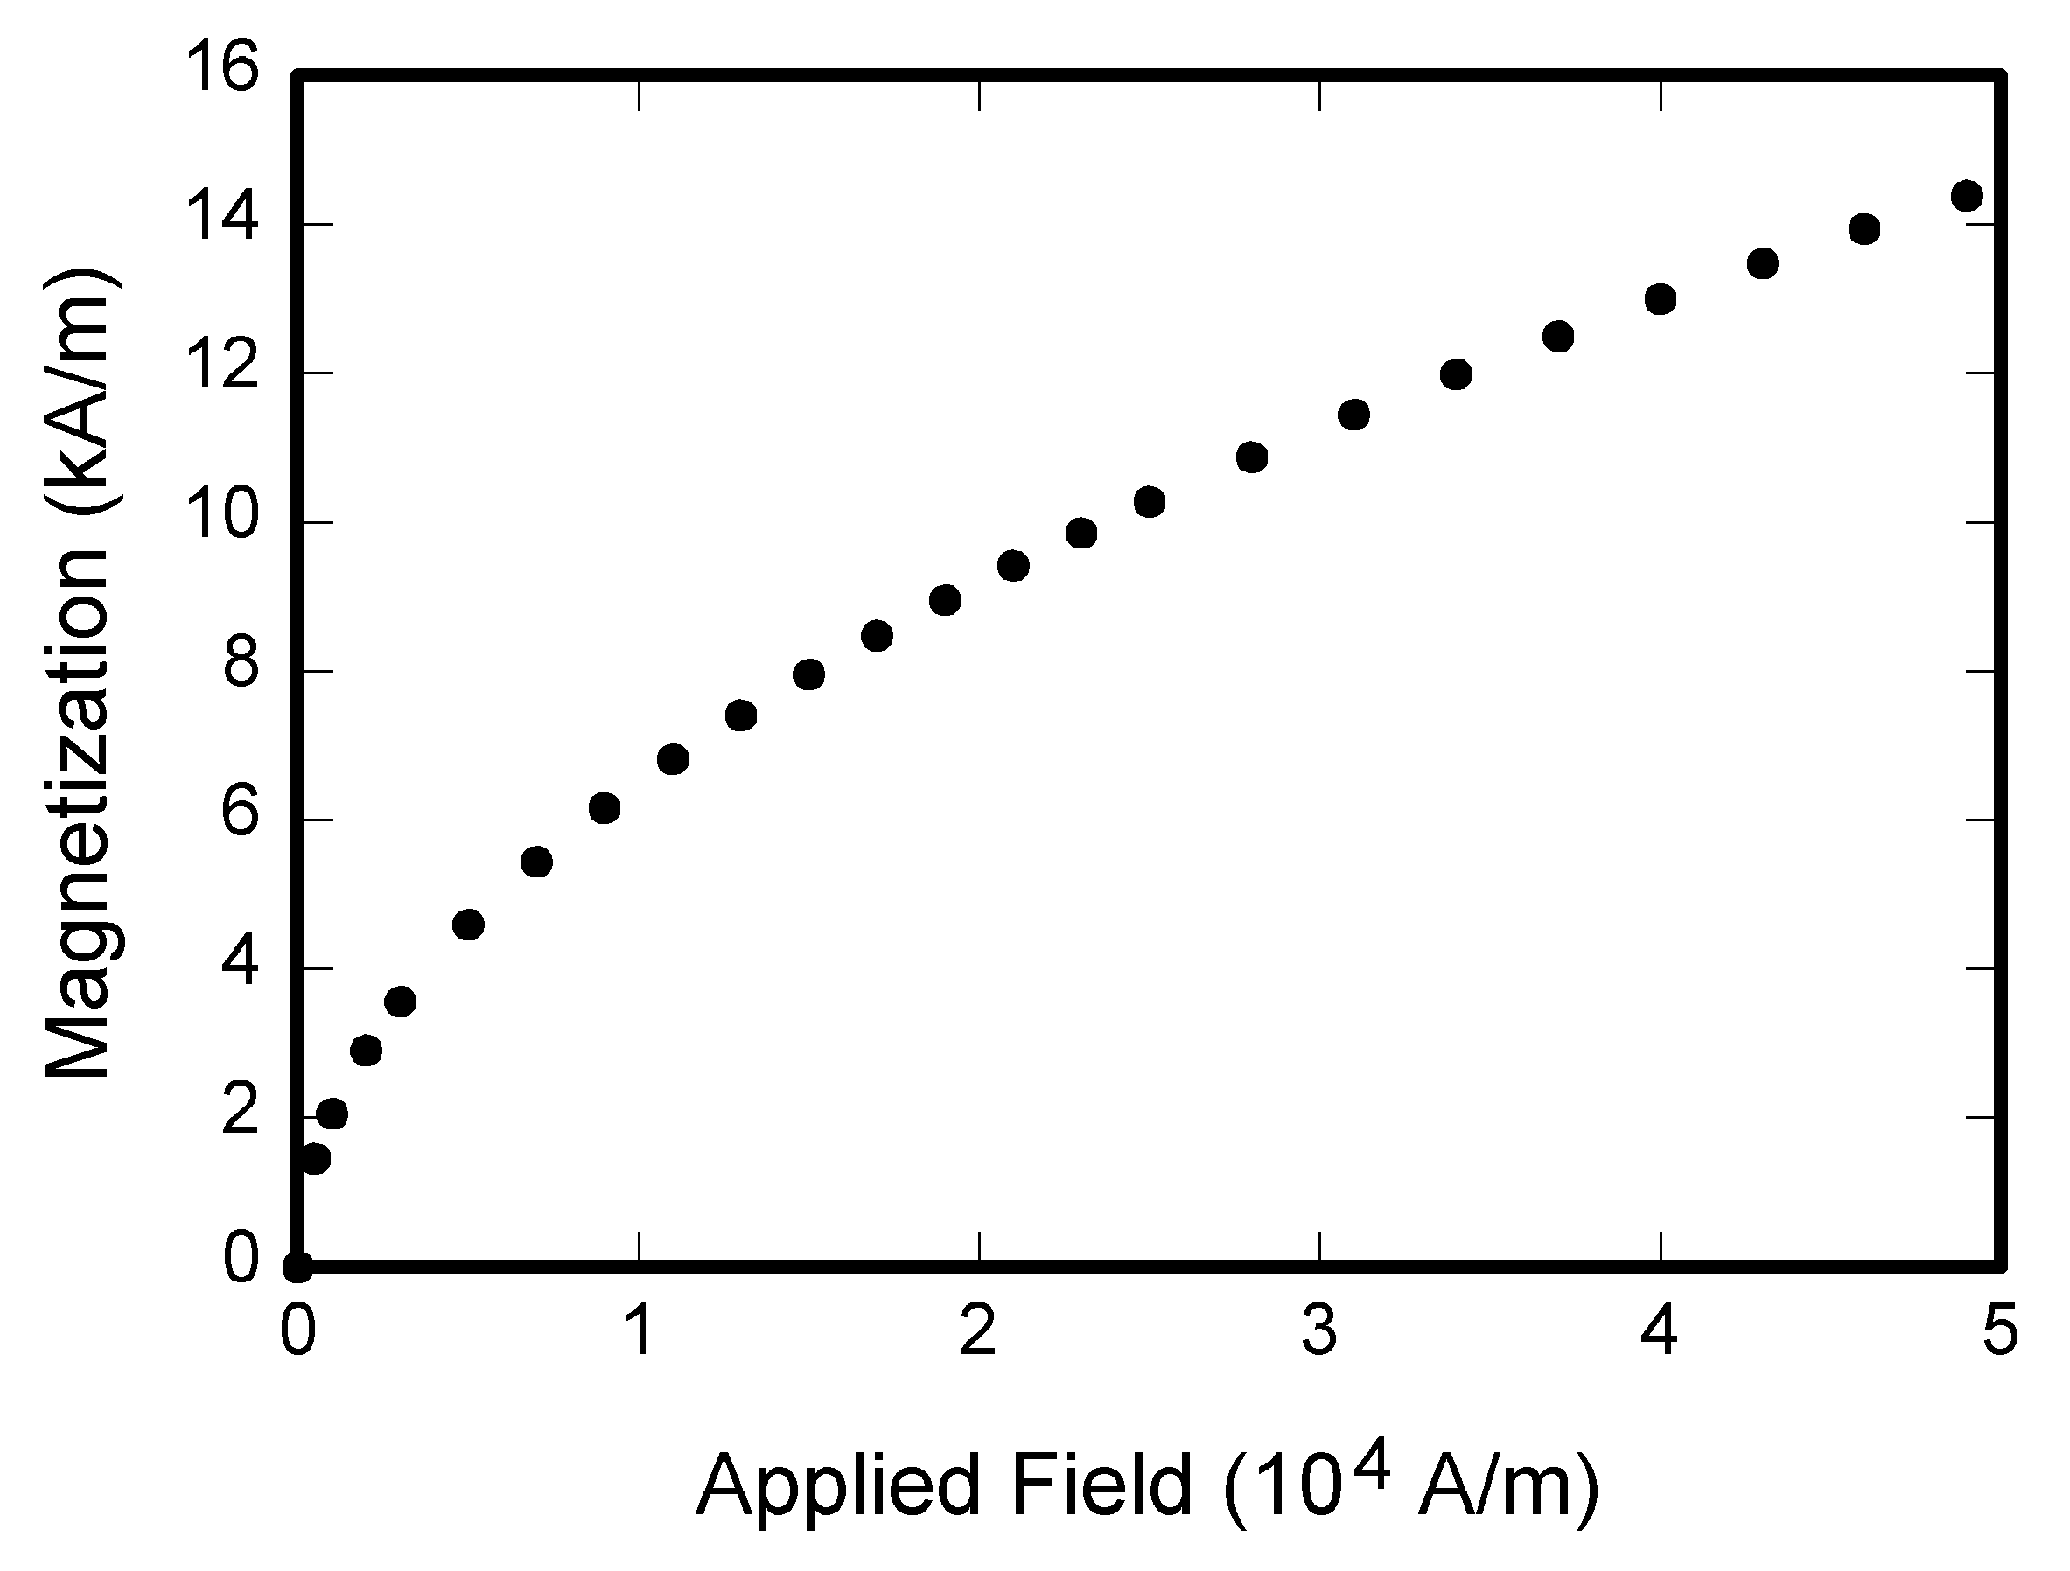
\includegraphics[width=7.16in]{Photos/fig1.png}
%     \caption{Example of a figure caption. - TWO Column}
%     \label{fig:name2}
% \end{figure}

\begin{figure*}[htbp]
    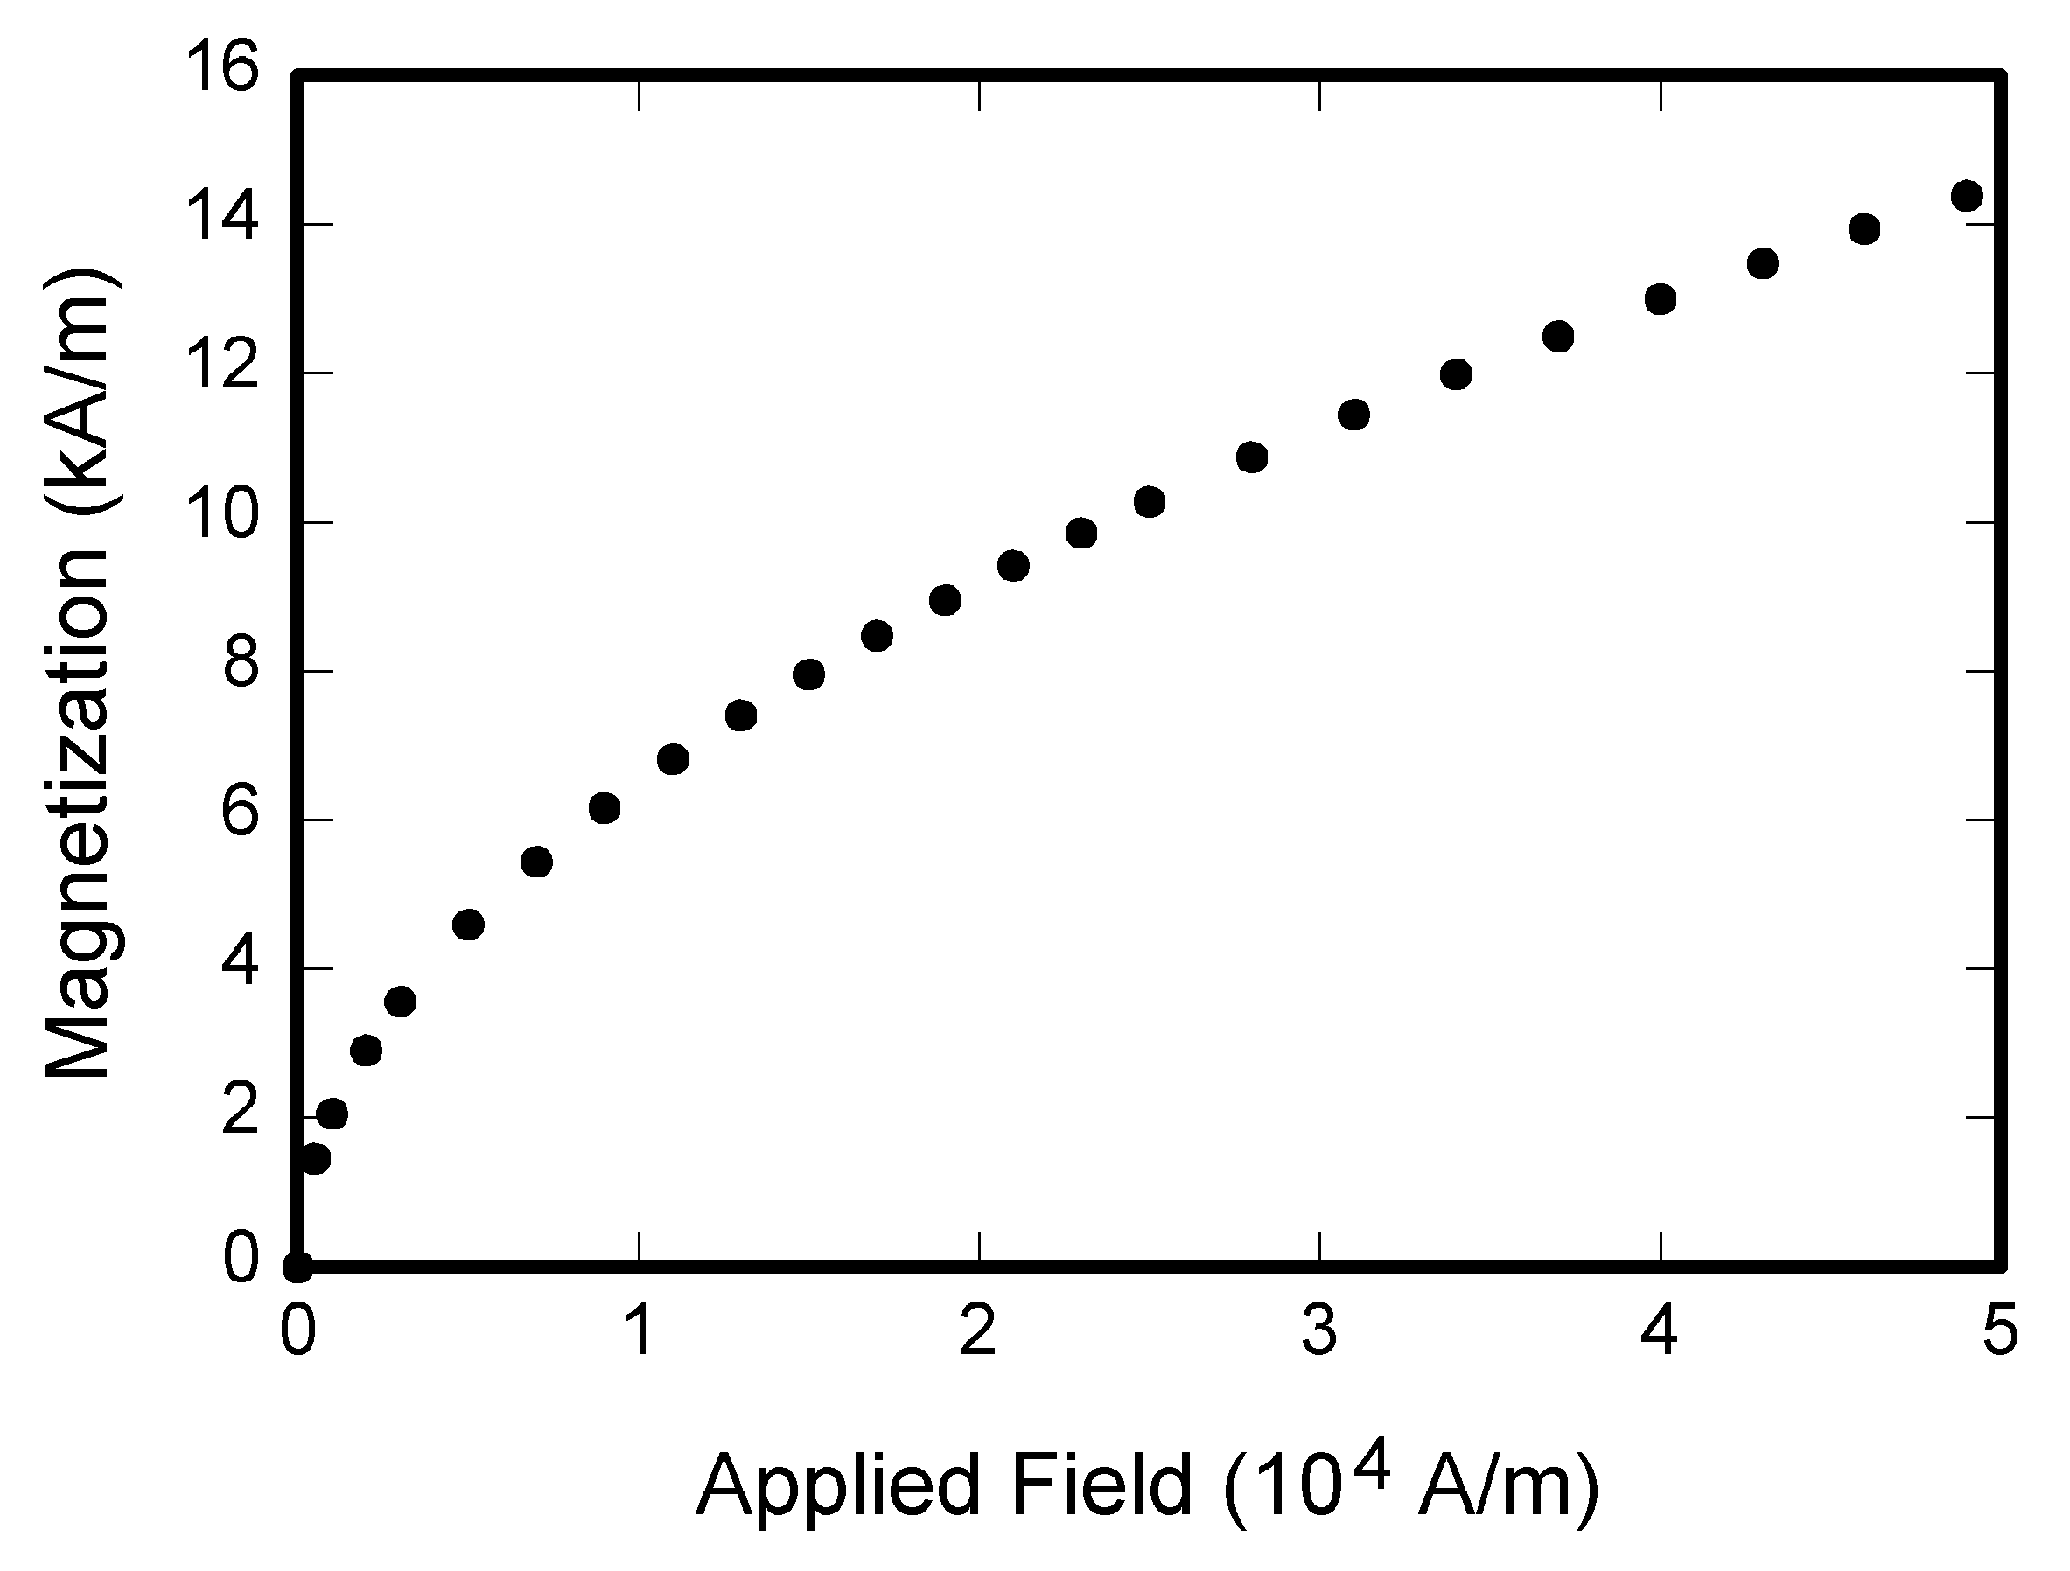
\includegraphics[width=\textwidth]{Photos/fig1.png}
    \caption{Example of a figure caption. - TWO Column}
    \label{fig:name3}
\end{figure*}

\begin{figure}[!h]
    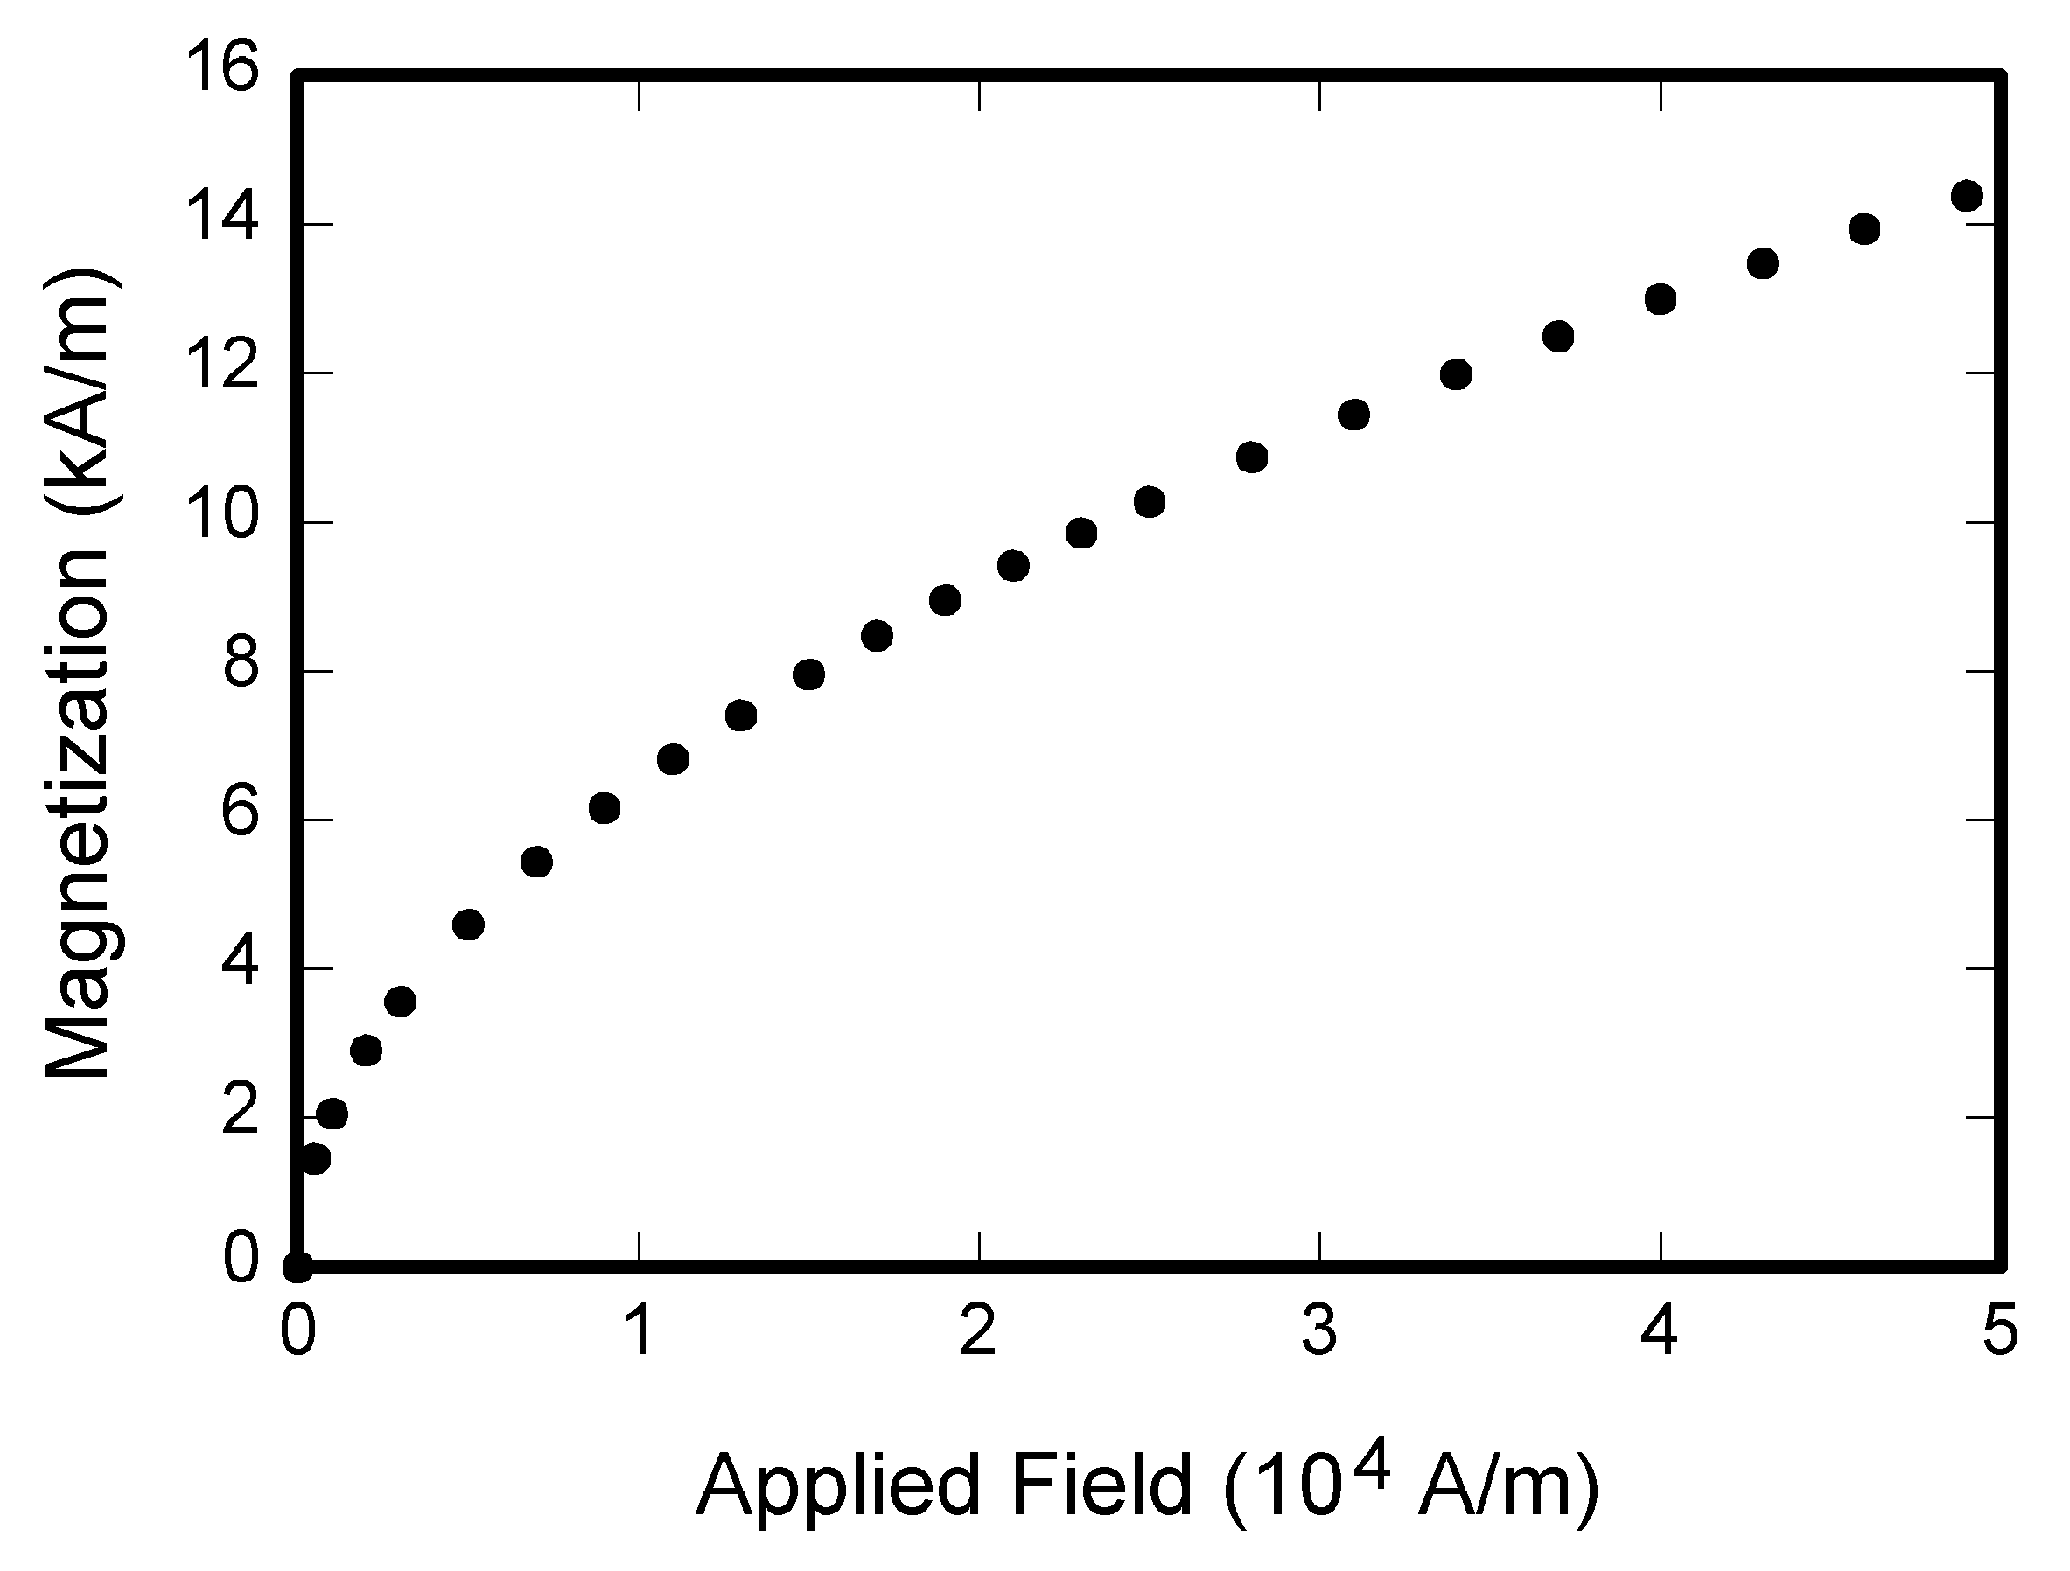
\includegraphics[width=\columnwidth]{Photos/fig1.png}
    \caption{Example of a figure caption. - ONE Column}
    \label{fig:name4}
\end{figure}

\begin{figure}[htbp] % Use subfig package
    \centering
    \subfloat[First image caption]{%
        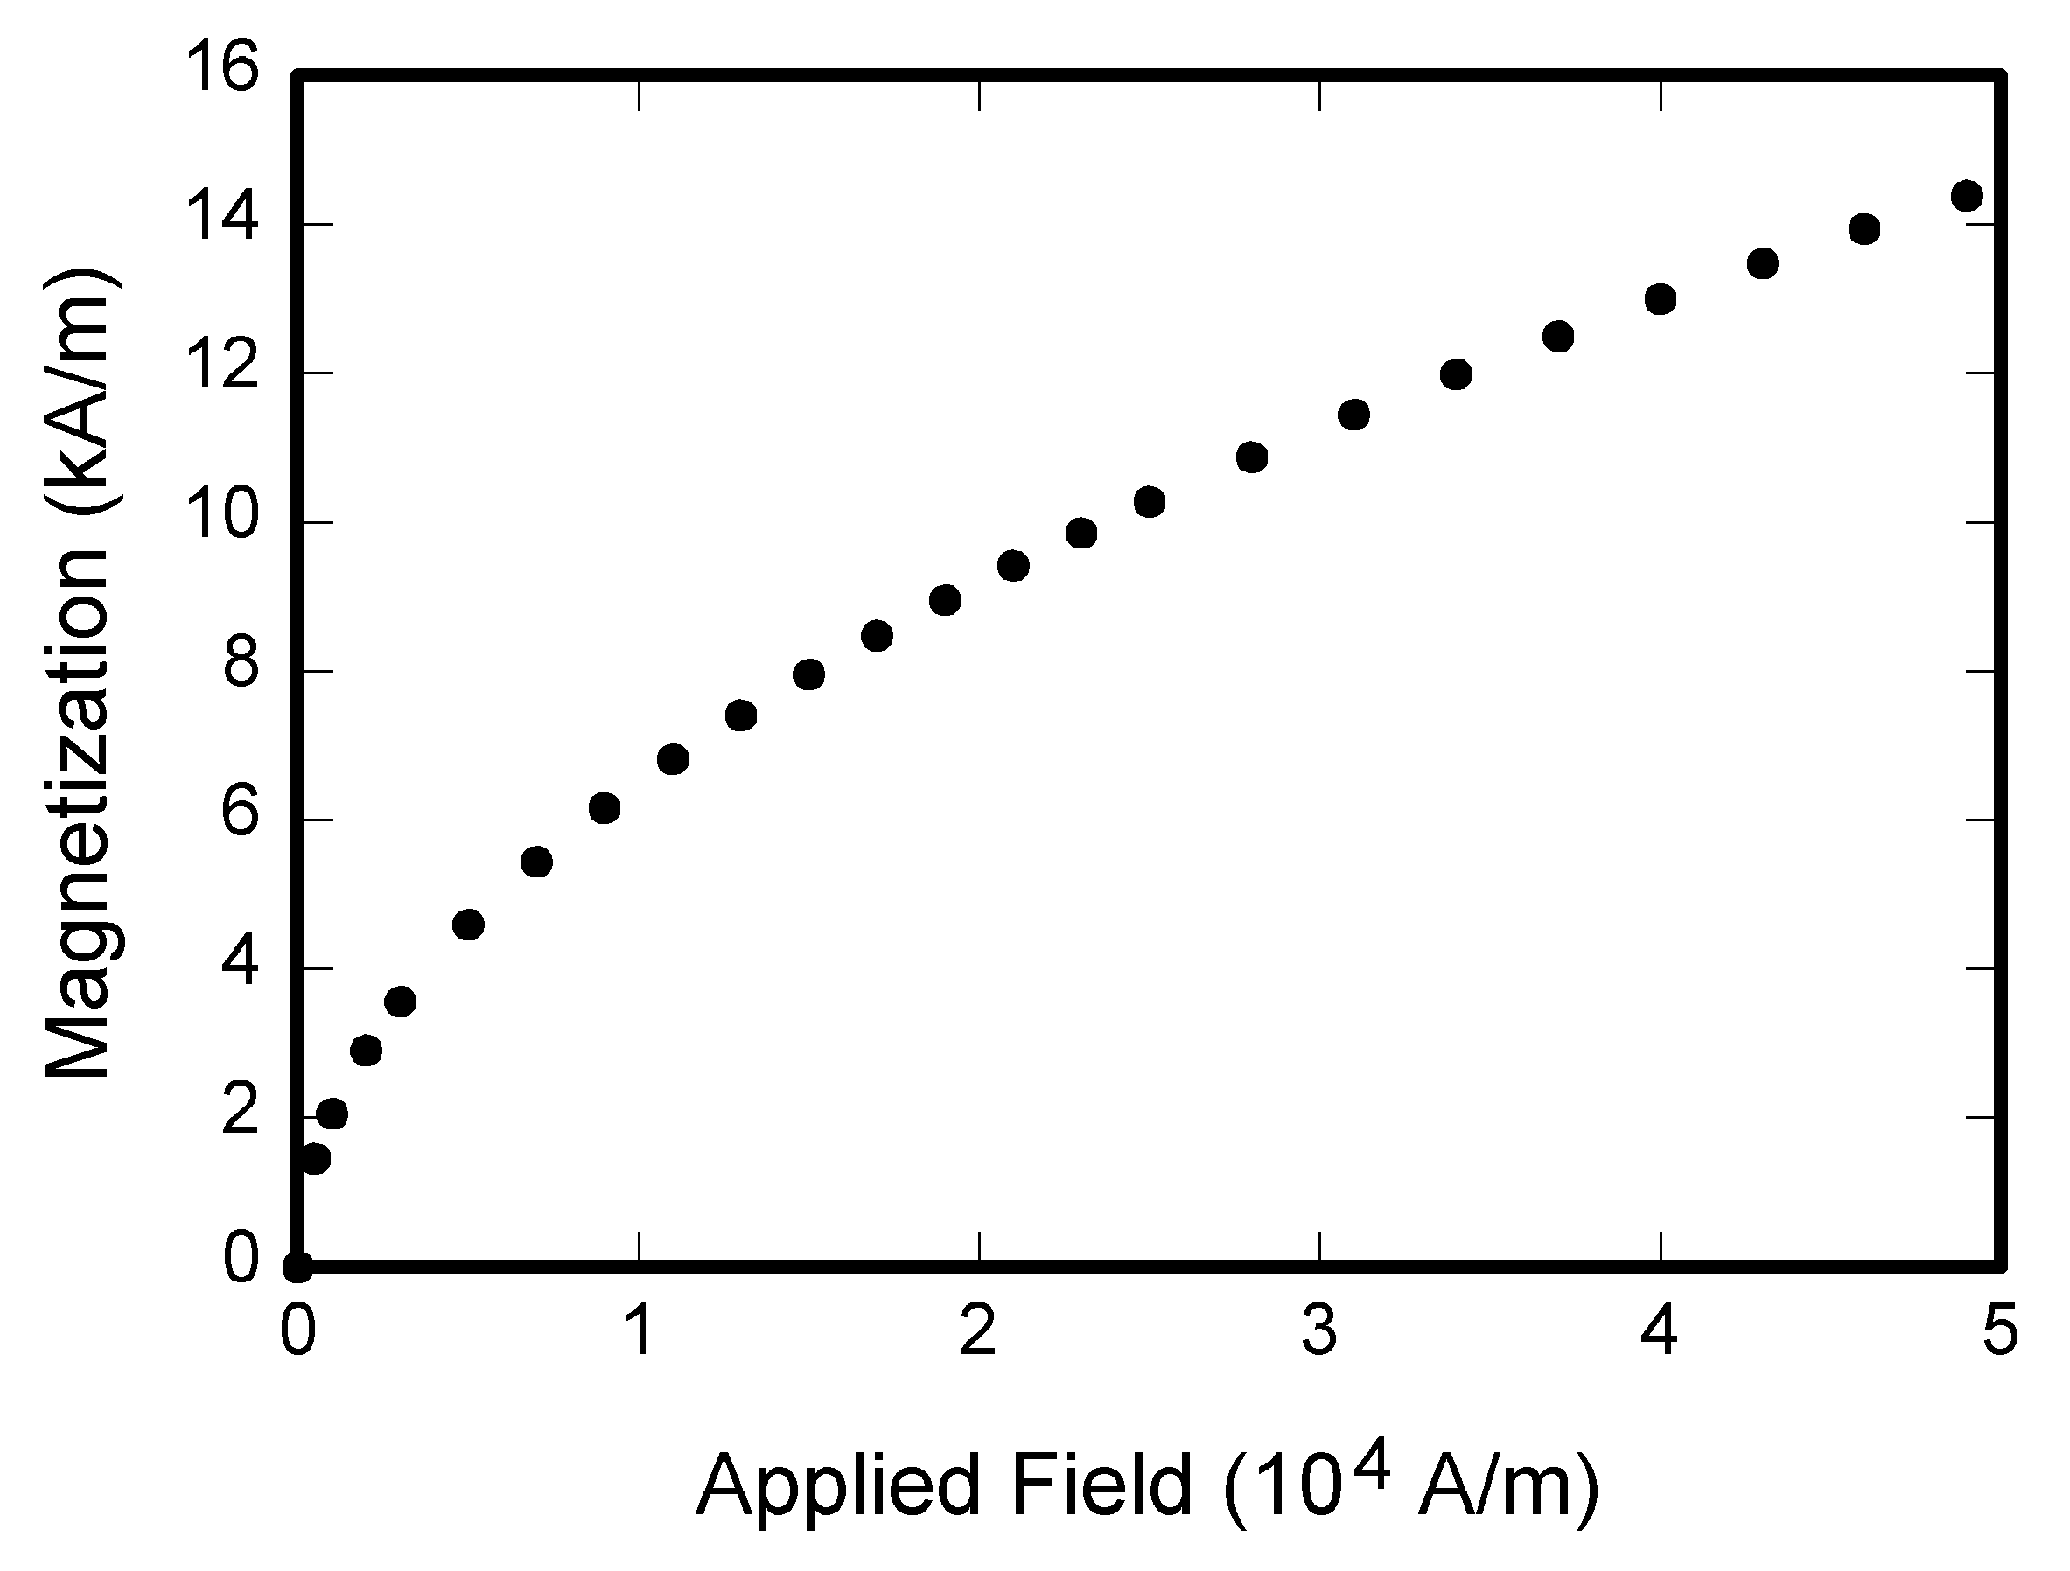
\includegraphics[width=0.45\columnwidth]{Photos/fig1.png}
        \label{fig:subfig1}
    }
    \hfill
    \subfloat[Second image caption]{%
        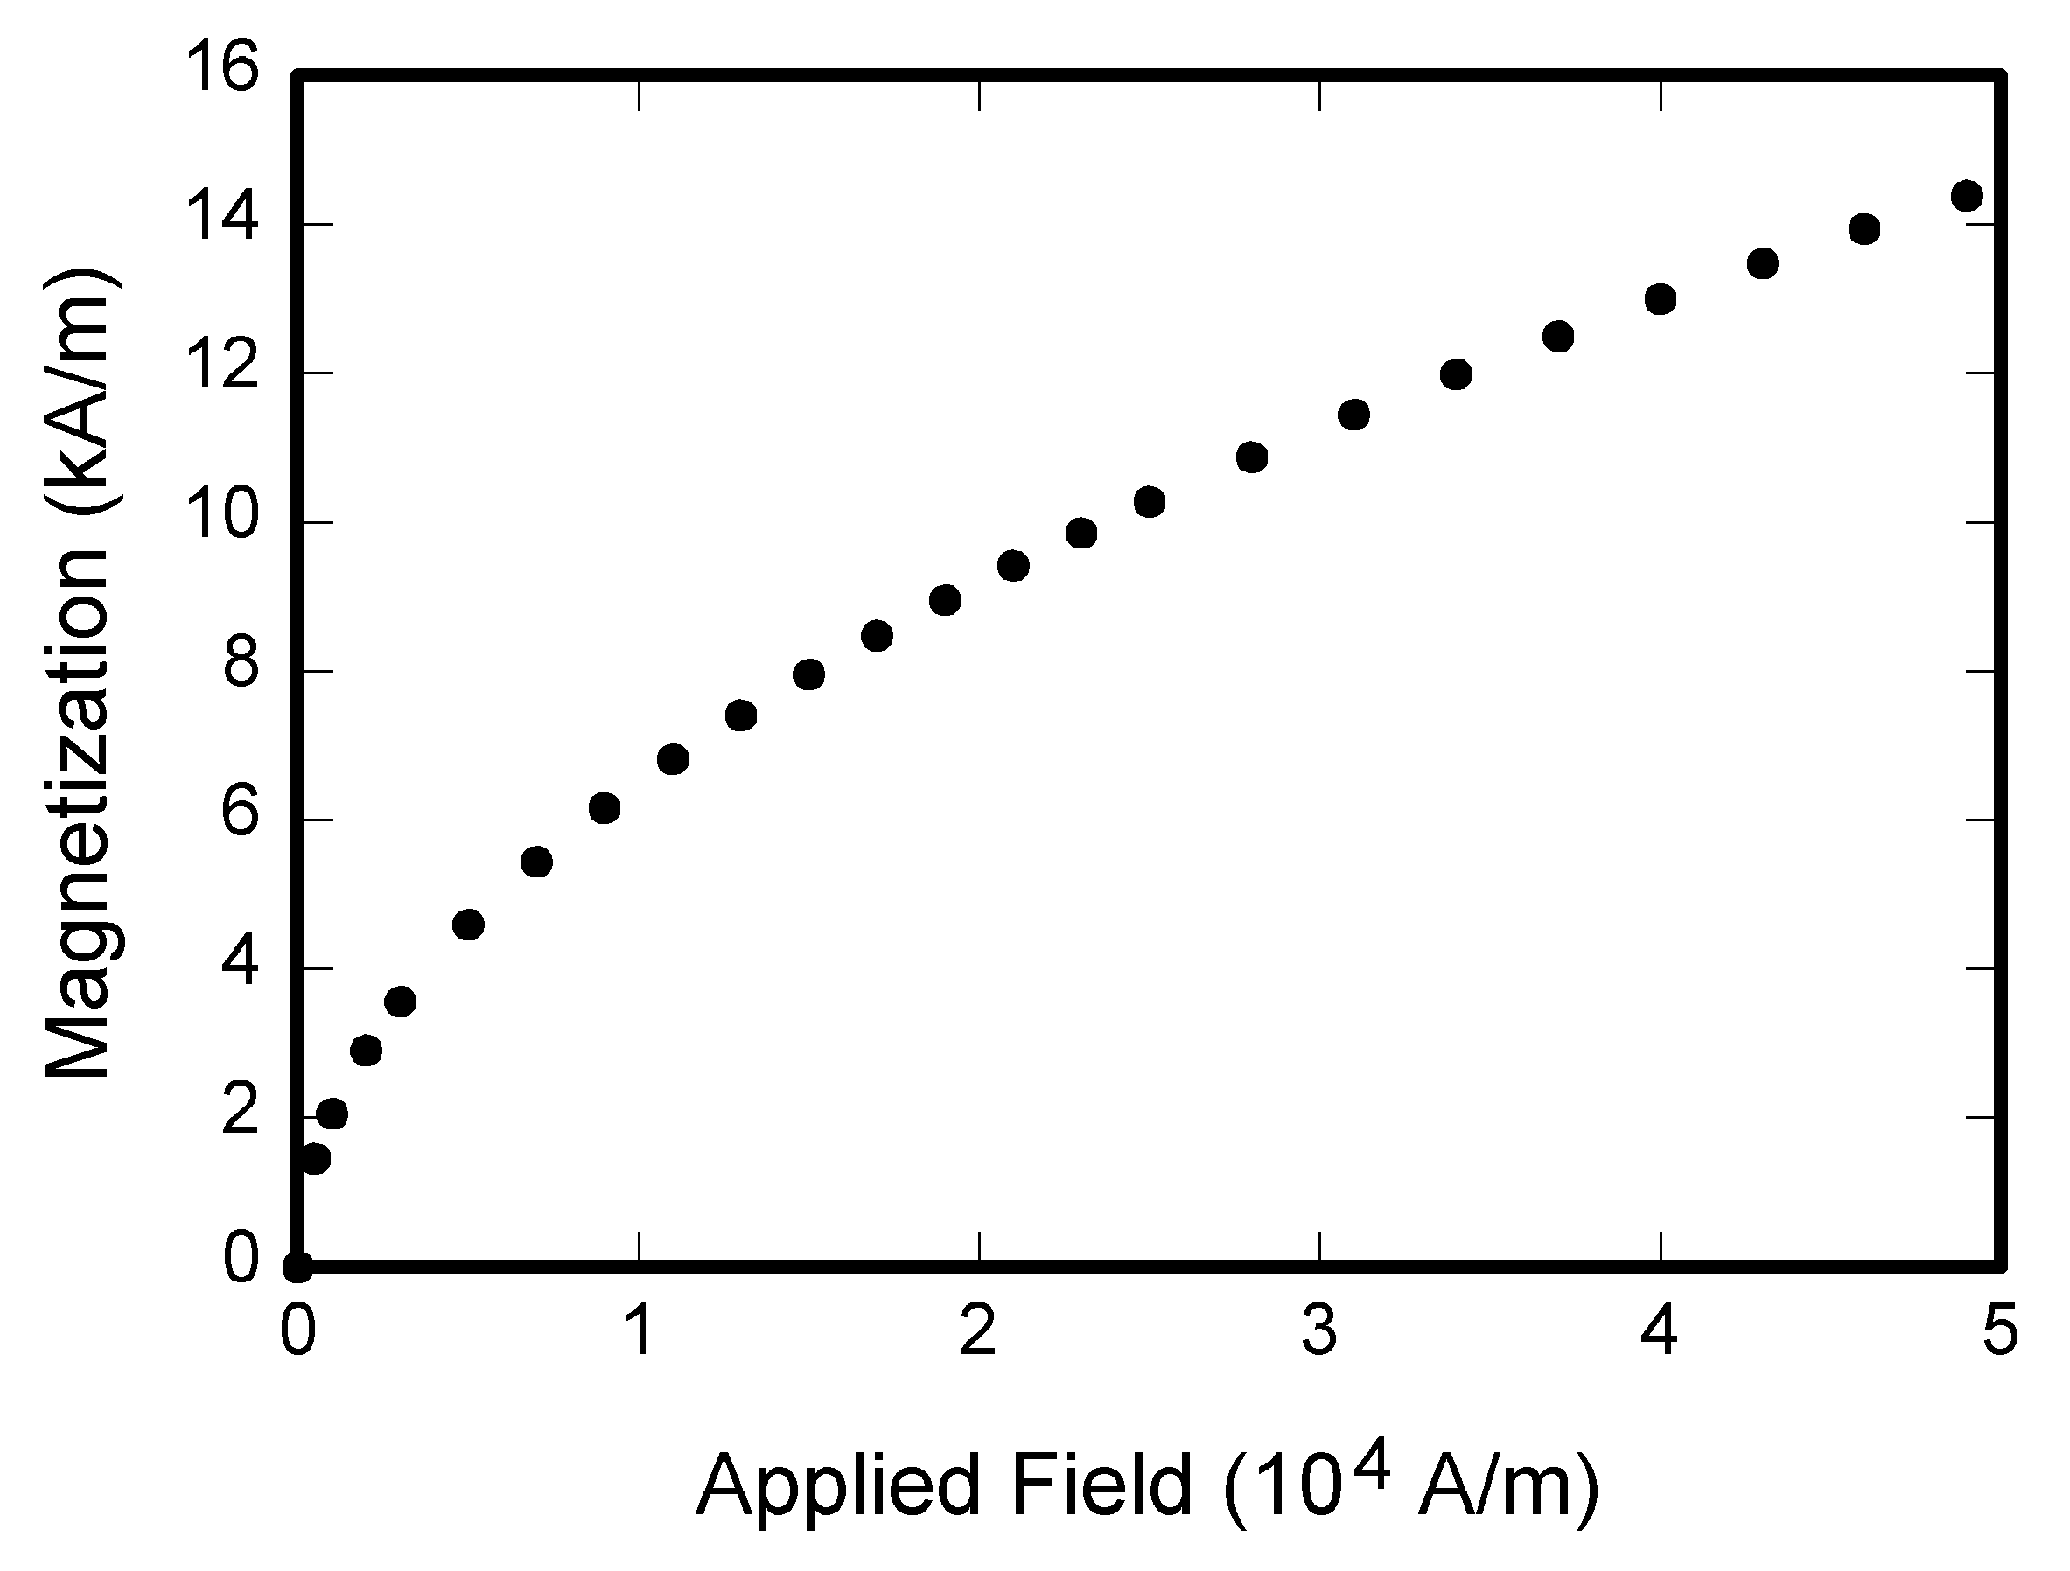
\includegraphics[width=0.45\columnwidth]{Photos/fig1.png}
        \label{fig:subfig2}
    }
    \caption{Example of two subfigures in one figure.}
    \label{fig:mainfig}
\end{figure}

\begin{figure}[htbp] % Use subcaption package
    \centering
    \begin{subfigure}{0.45\columnwidth}
        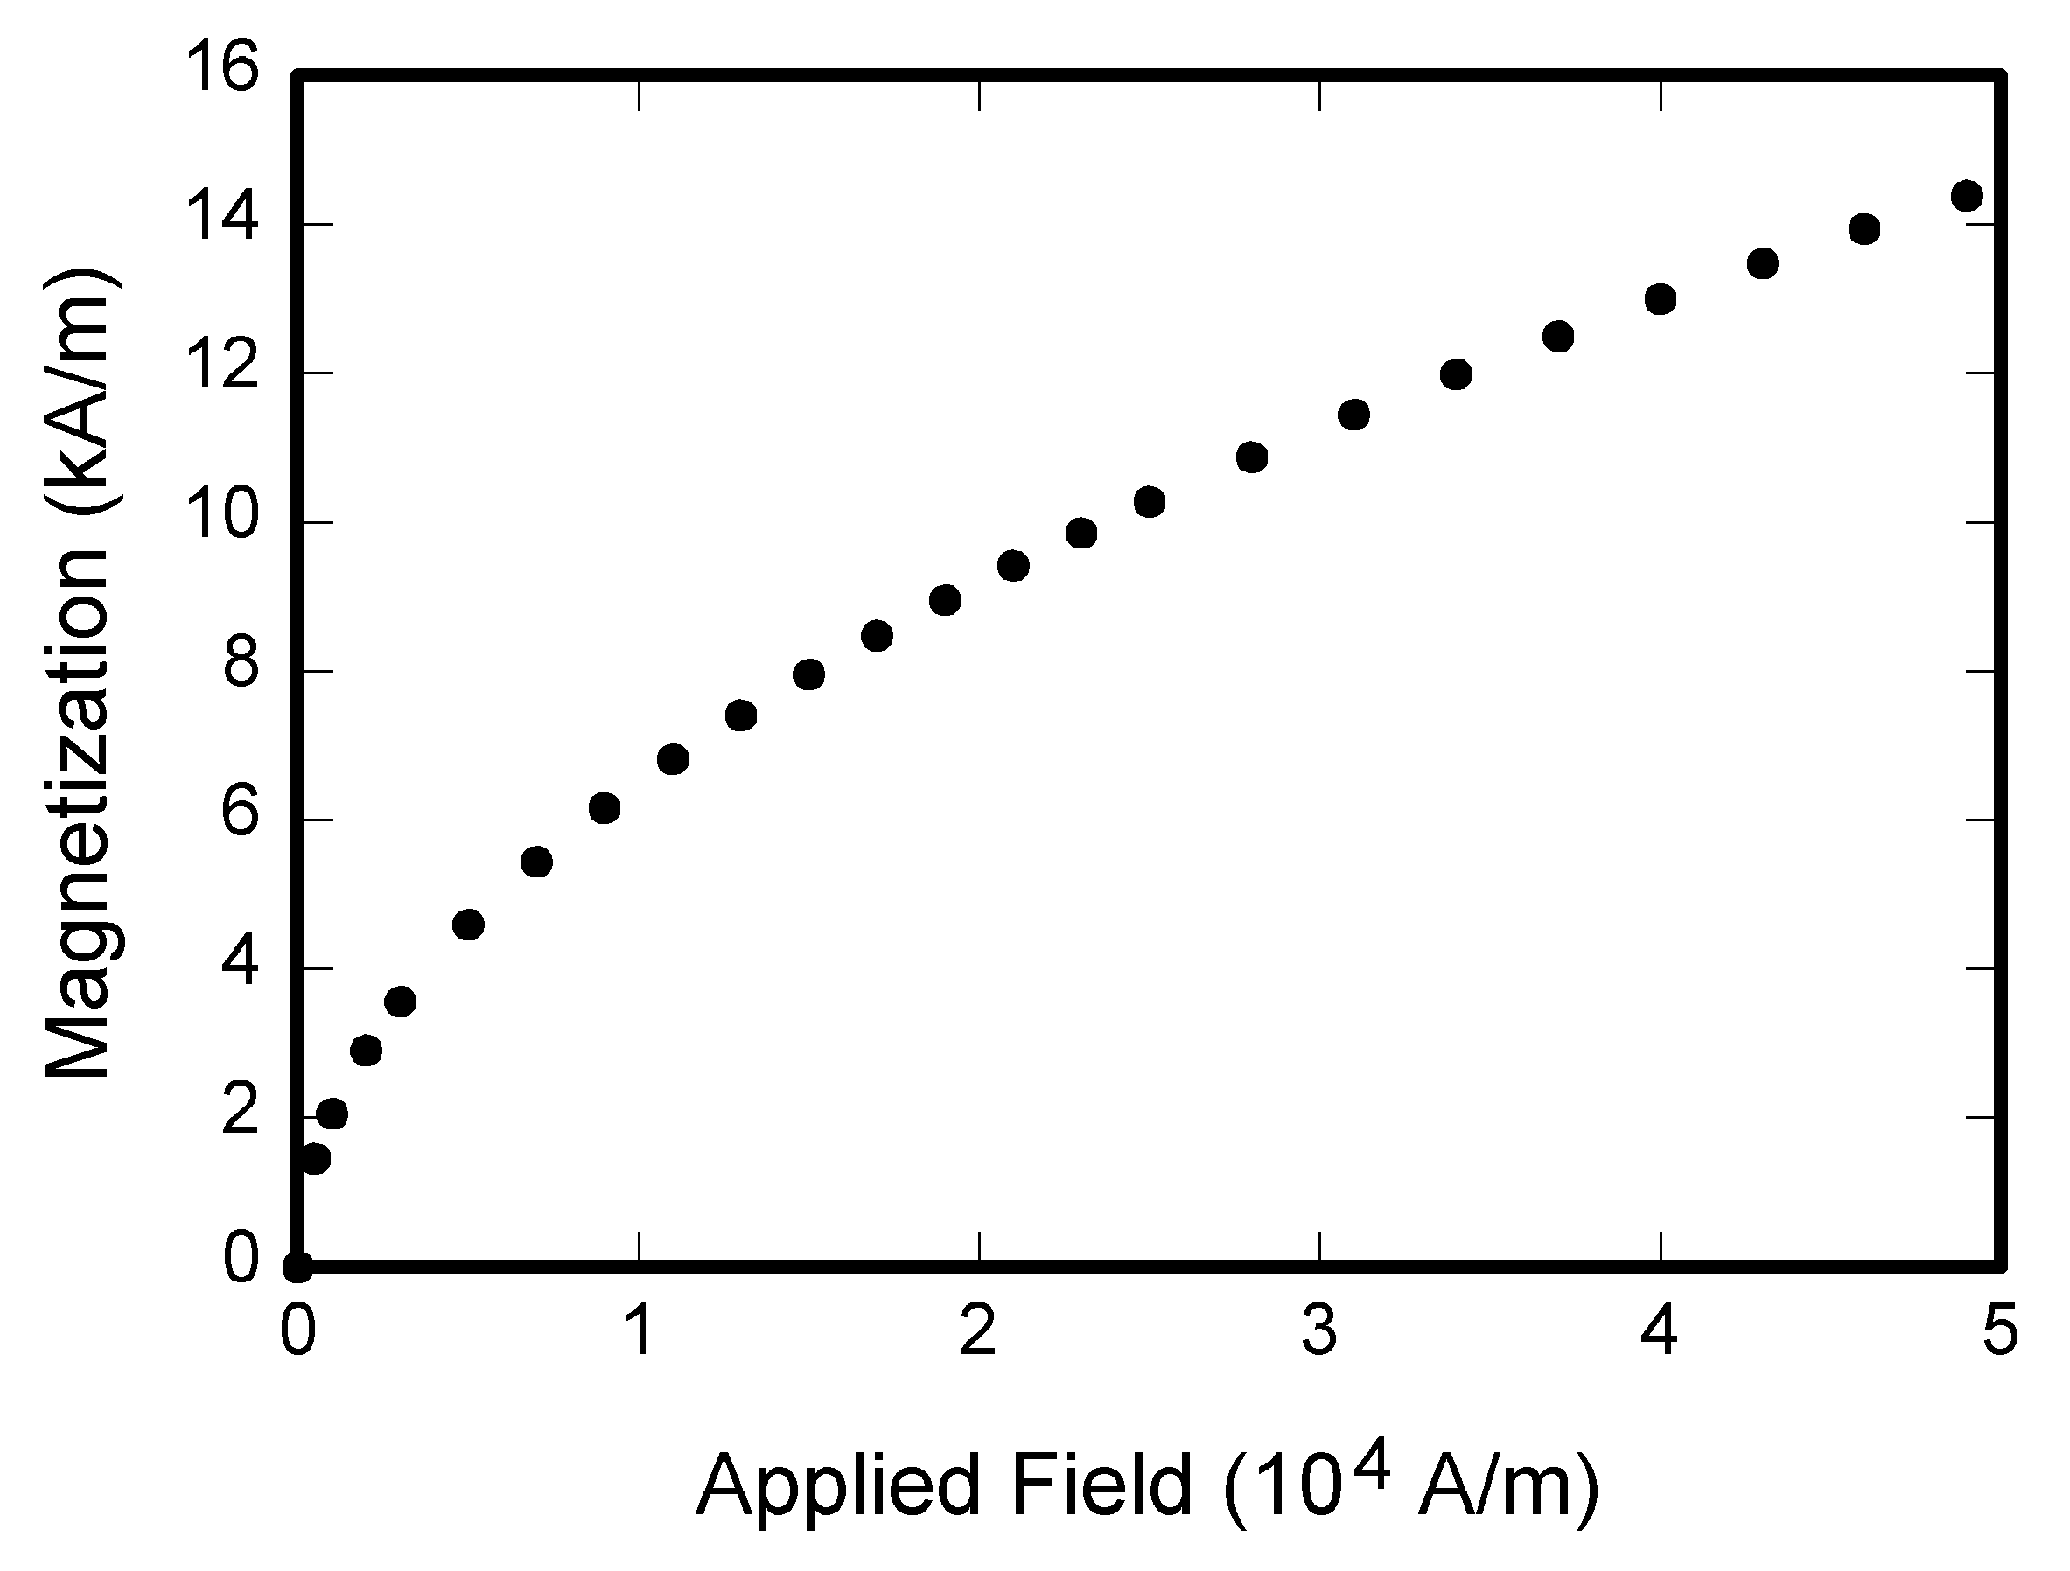
\includegraphics[width=\linewidth]{Photos/fig1.png}
        \caption{First image caption}
    \end{subfigure}
    \hfill
    \begin{subfigure}{0.45\columnwidth}
        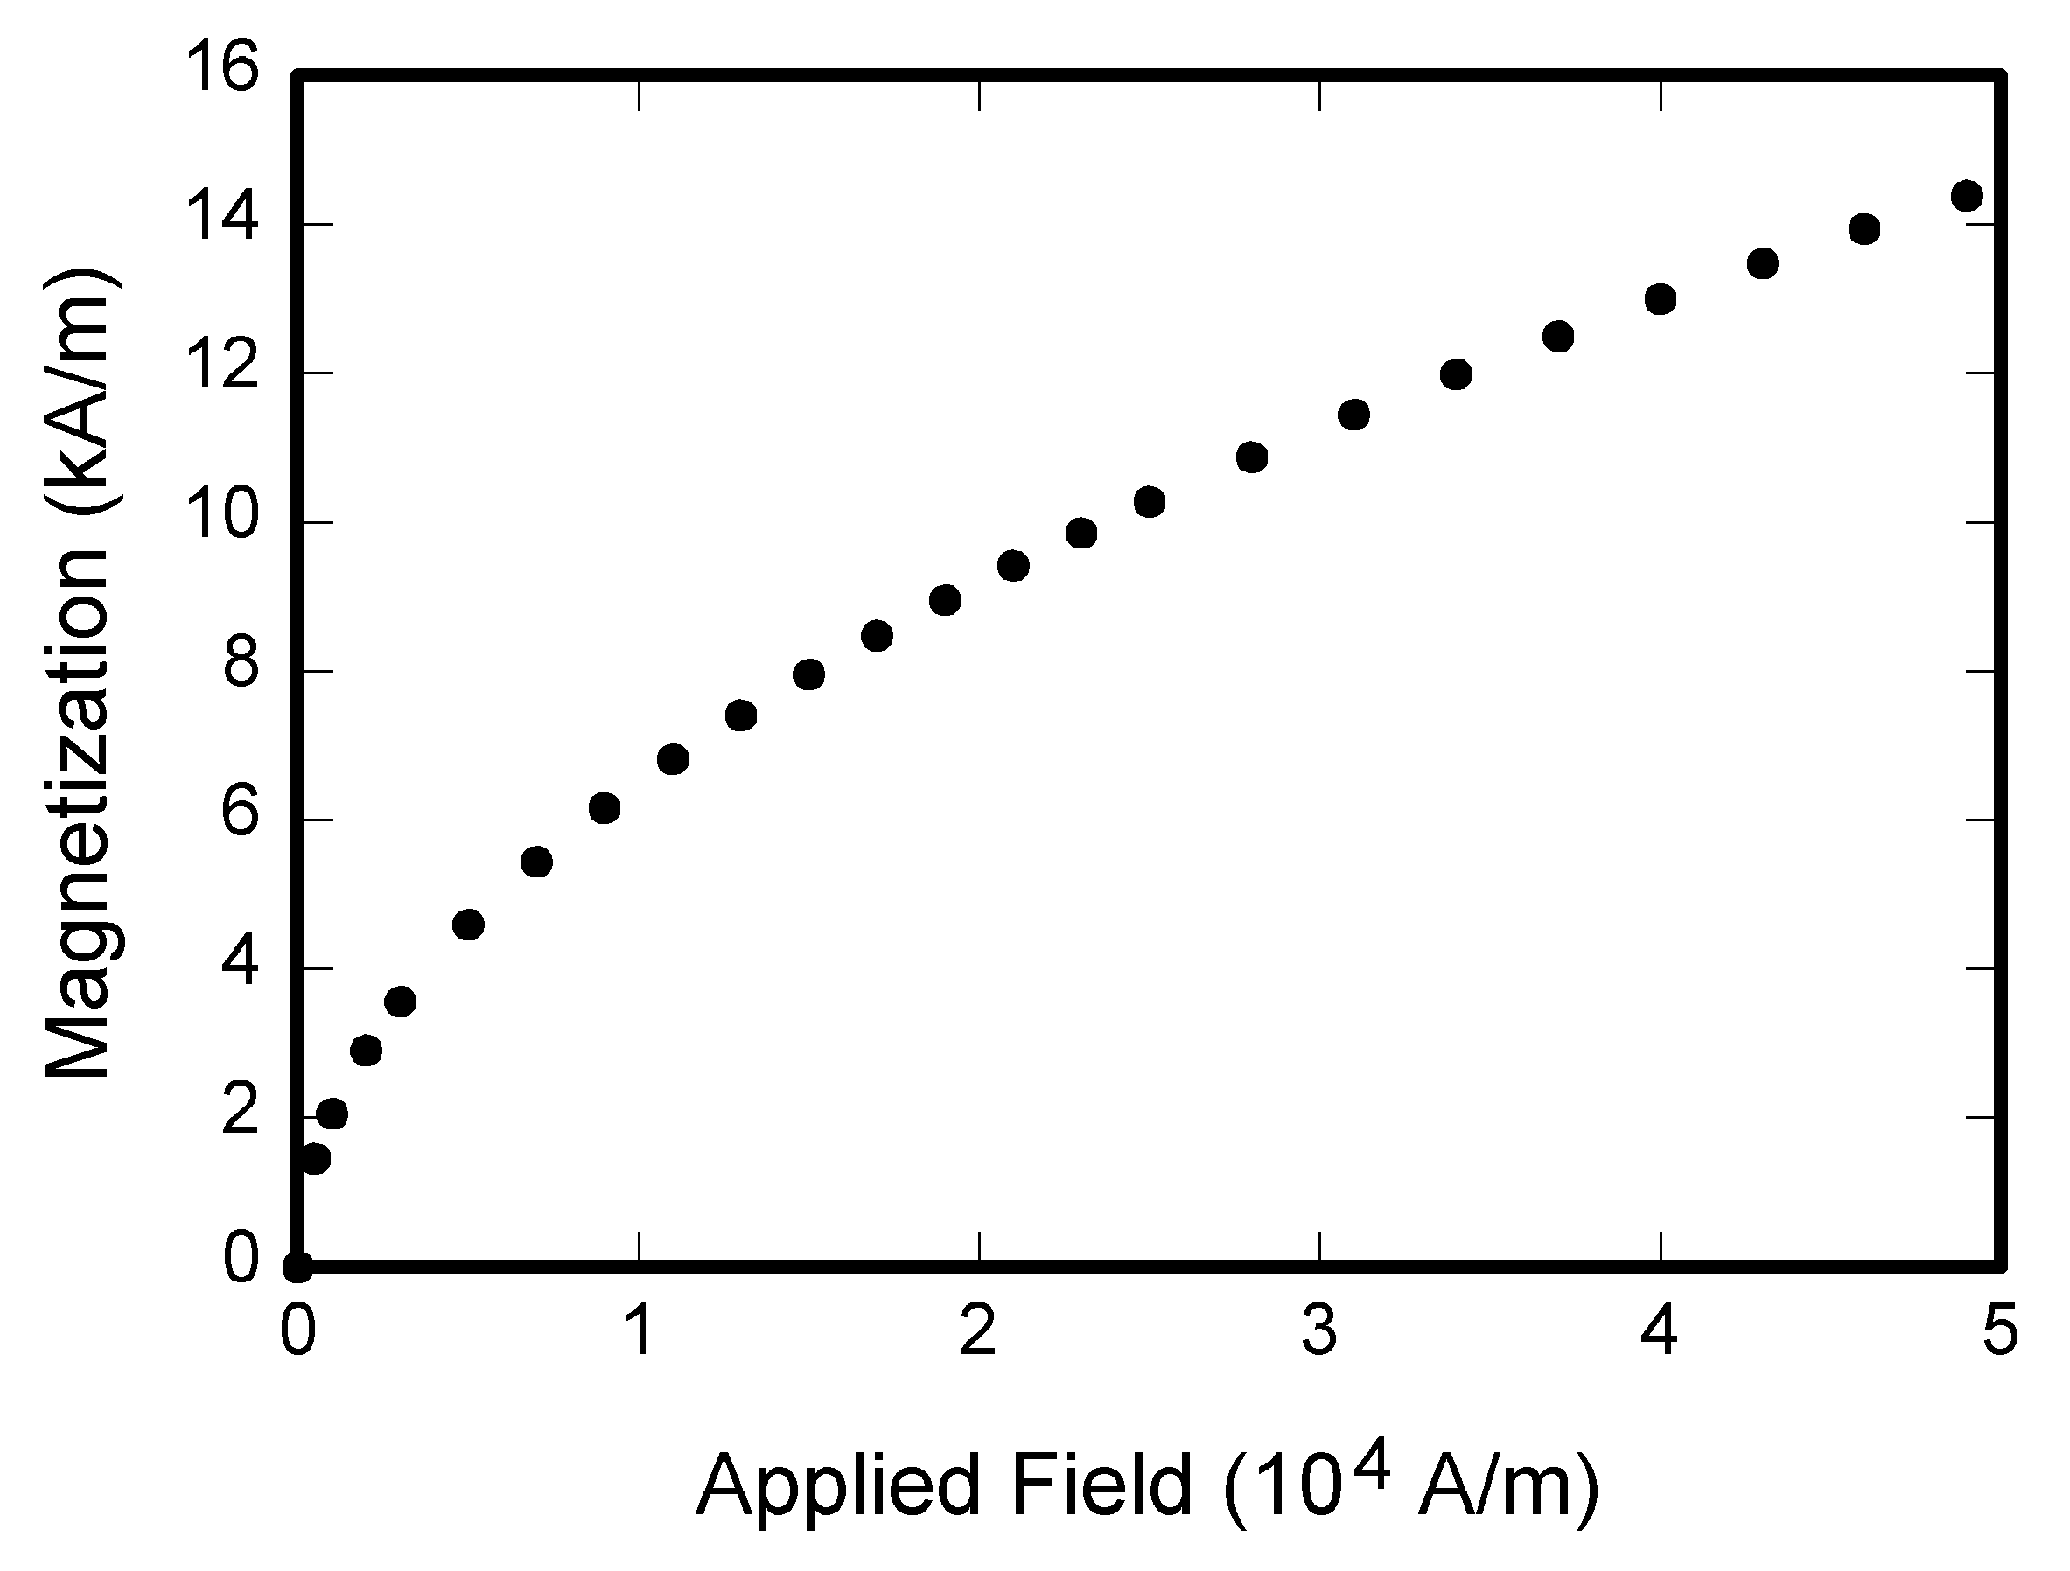
\includegraphics[width=\linewidth]{Photos/fig1.png}
        \caption{Second image caption}
    \end{subfigure}
    \caption{Example of two subfigures in one figure.}
    \label{fig:mainfig}
\end{figure}

\begin{figure}[htbp] % Use subcaption package
    \centering
    % --- First row ---
    \begin{subfigure}{0.45\columnwidth}
        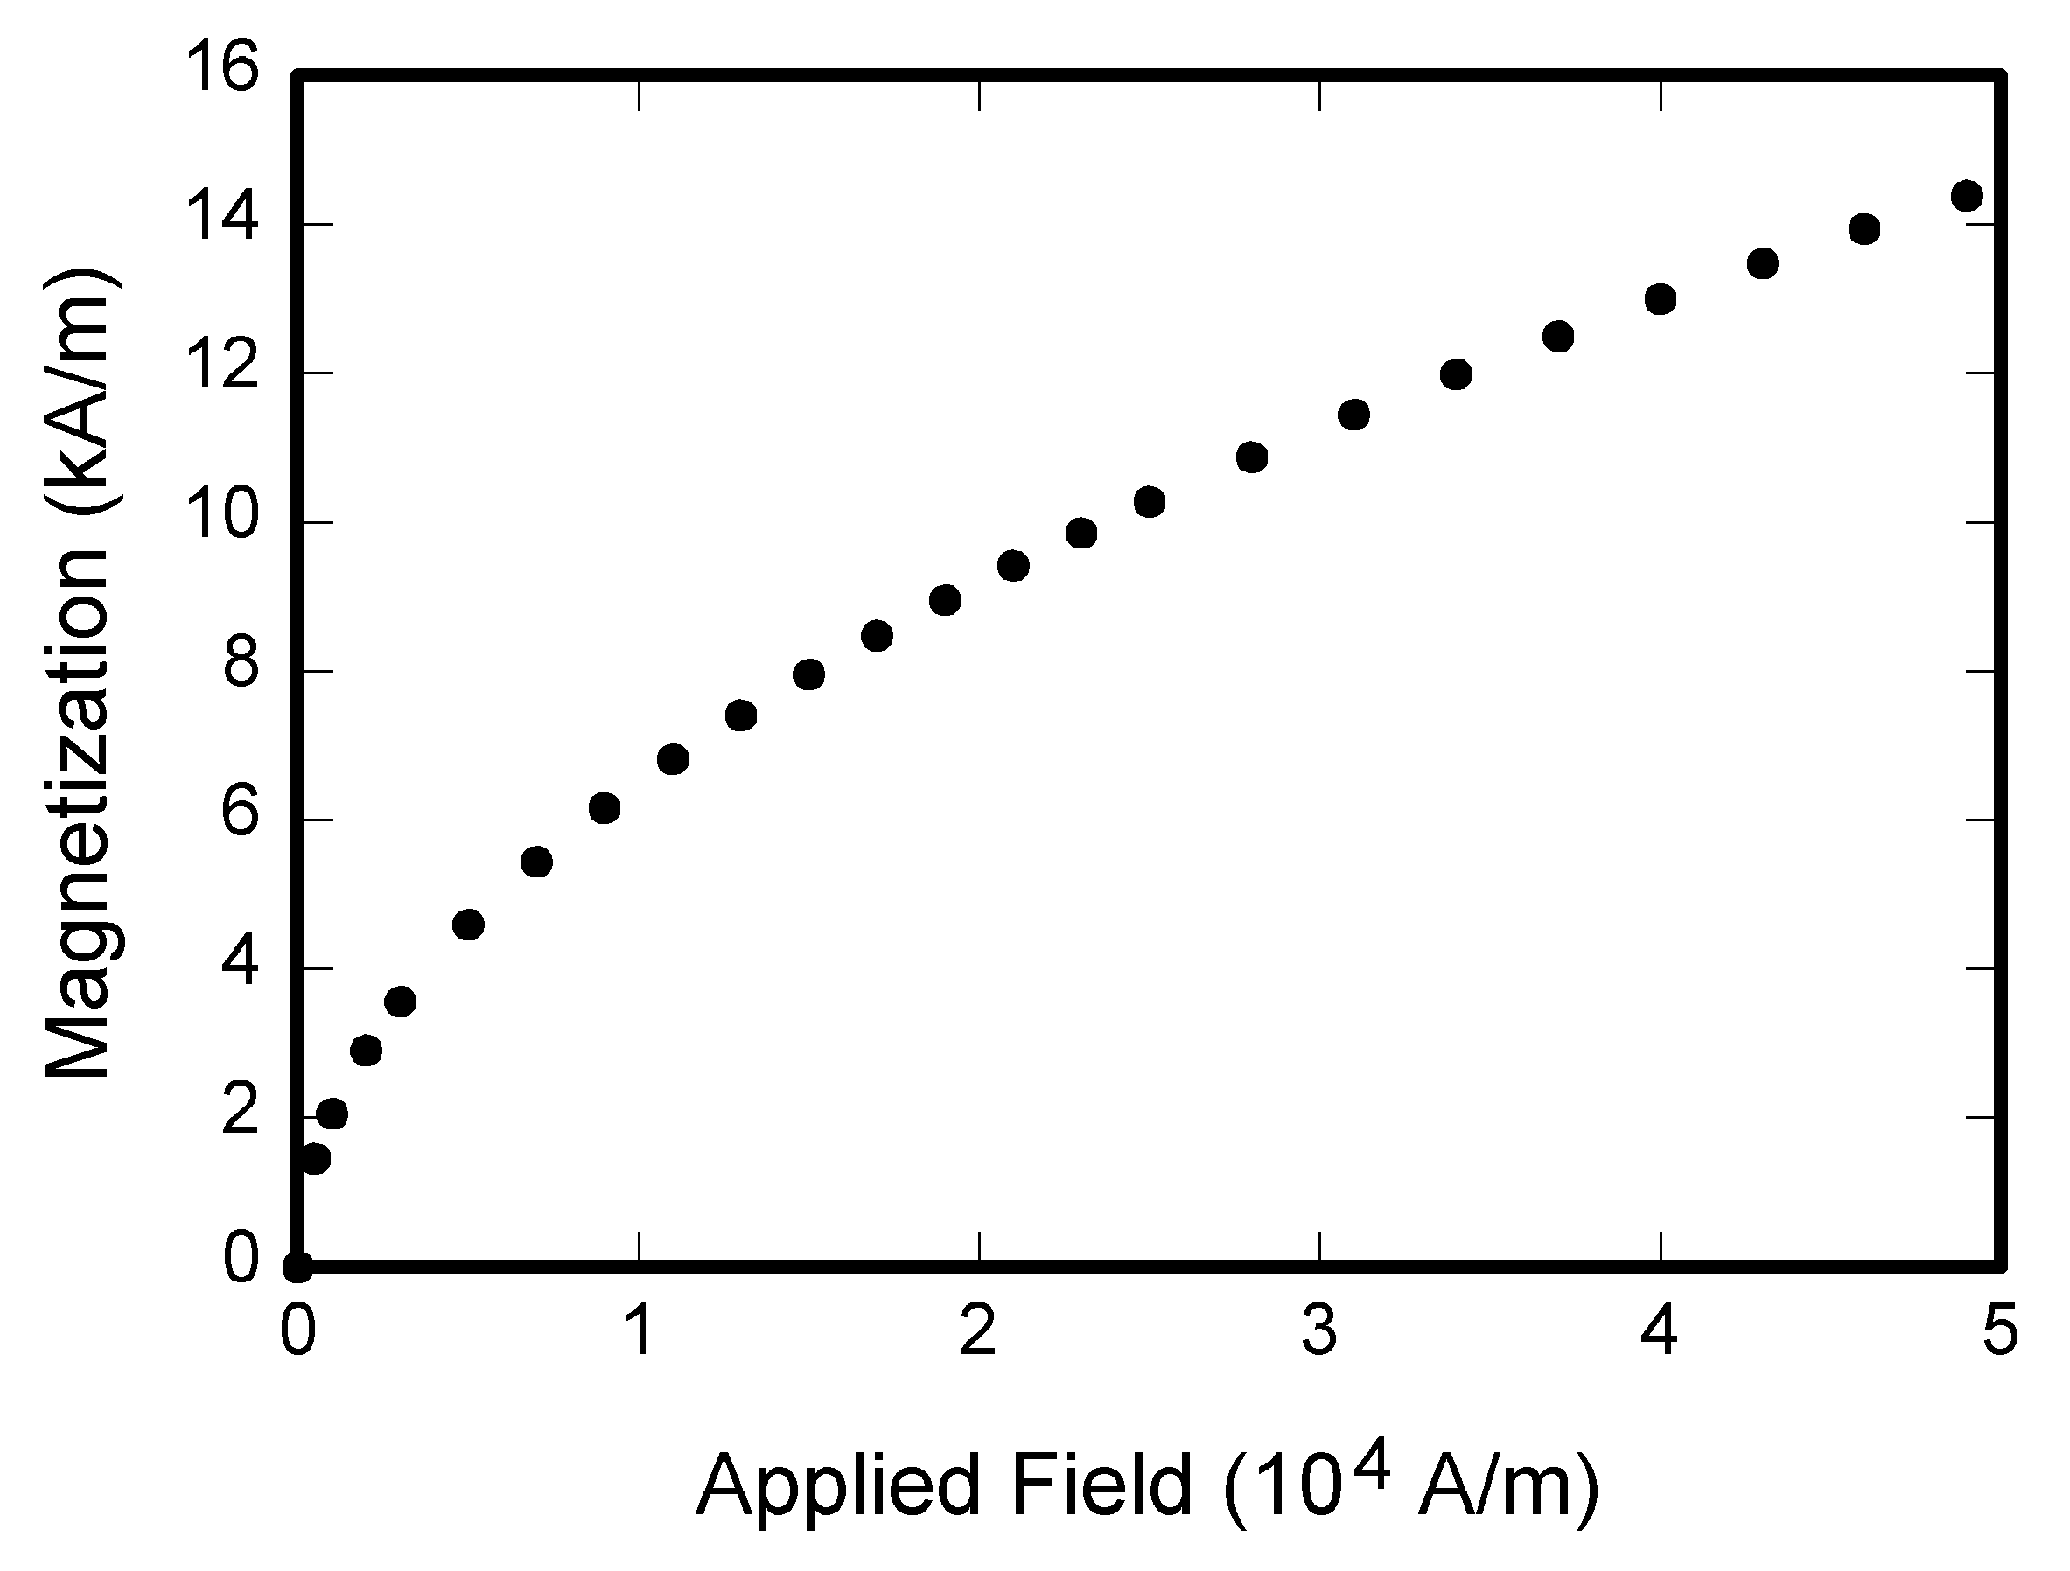
\includegraphics[width=\linewidth]{Photos/fig1.png}
        \caption{Caption 1}
        \label{fig:2a}
    \end{subfigure}\hfill
    \begin{subfigure}{0.45\columnwidth}
        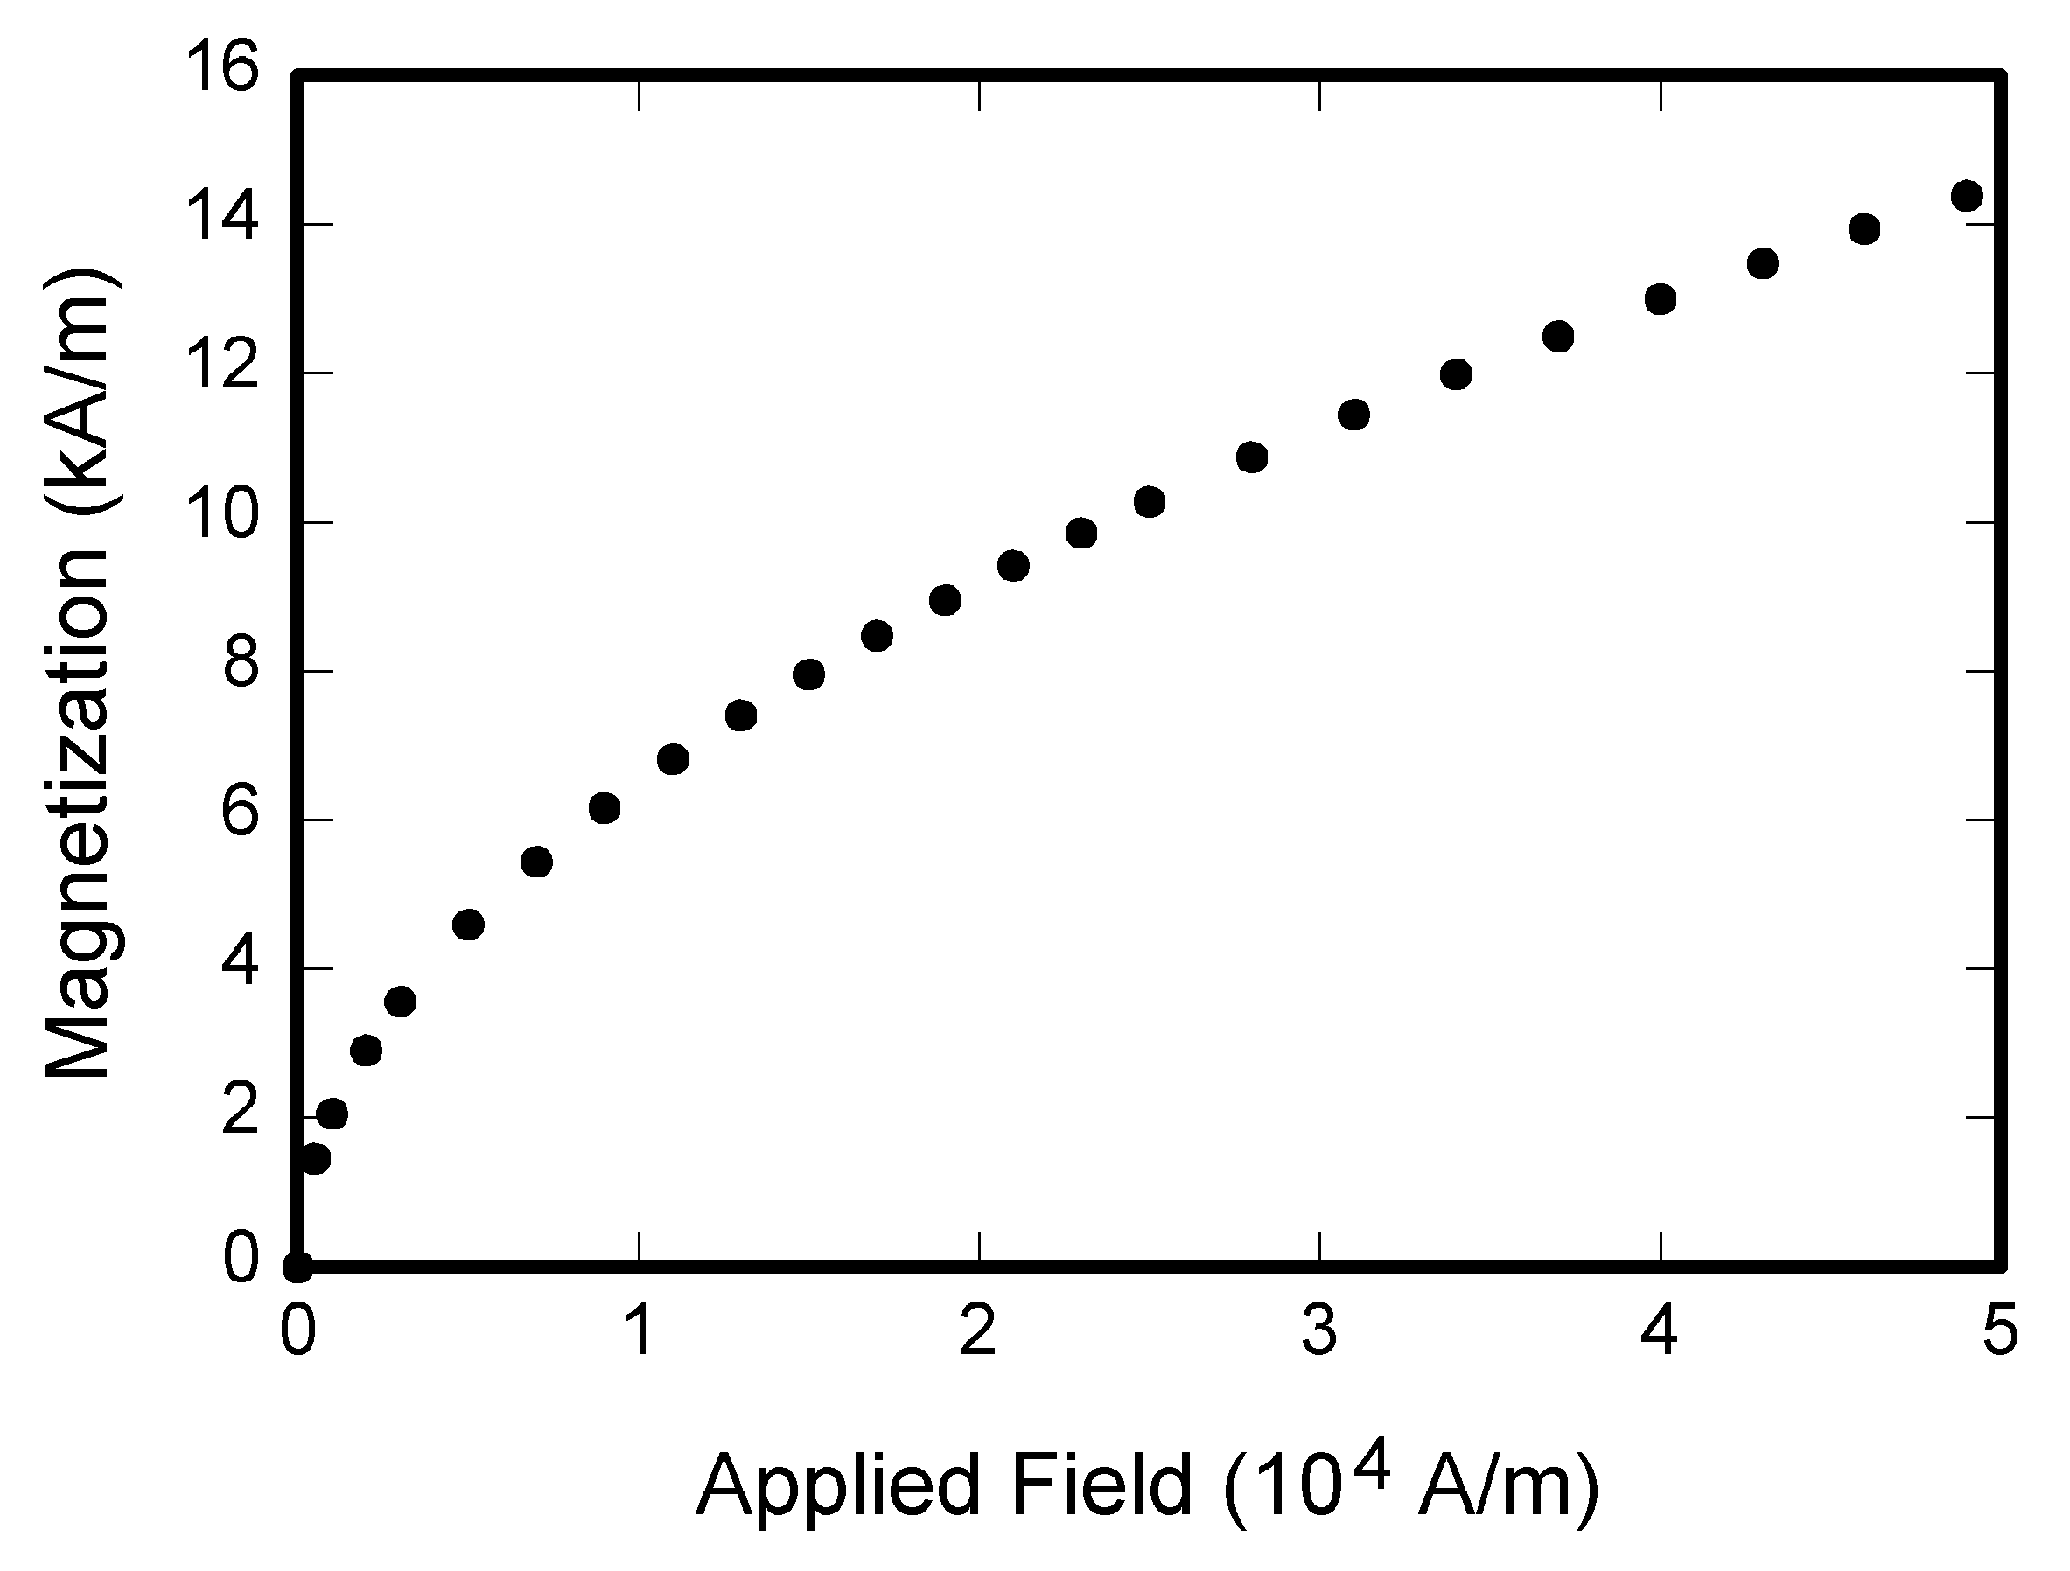
\includegraphics[width=\linewidth]{Photos/fig1.png}
        \caption{Caption 2}
        \label{fig:2b}
    \end{subfigure}

    % --- Second row ---
    \begin{subfigure}{0.45\columnwidth}
        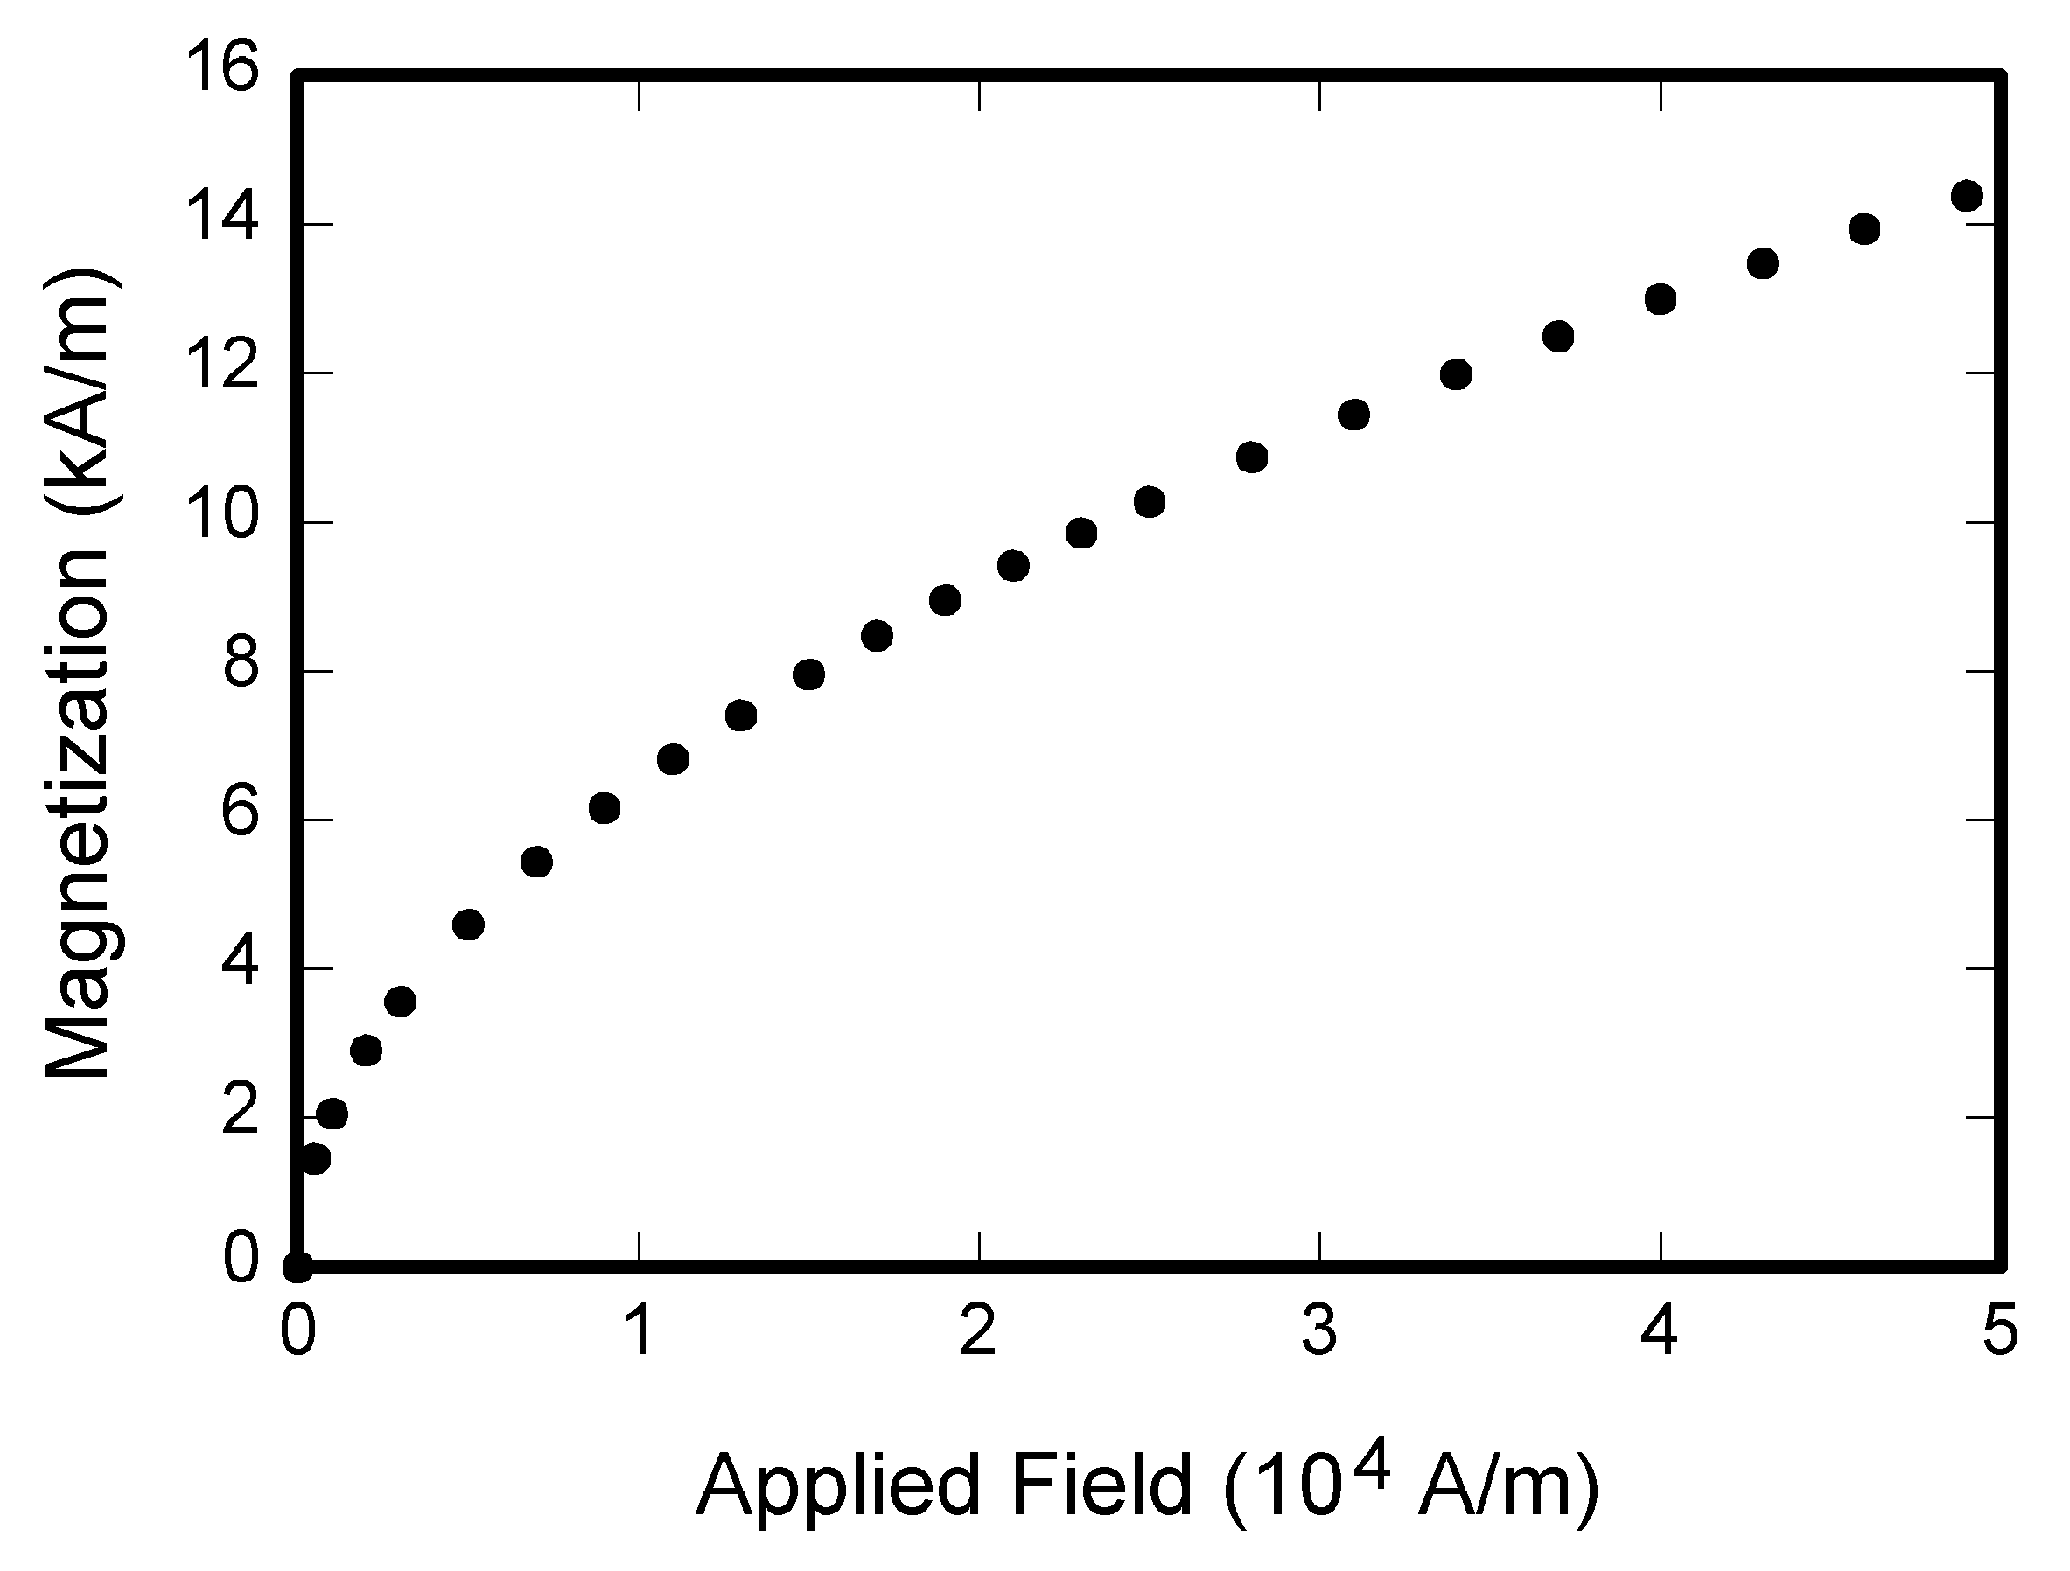
\includegraphics[width=\linewidth]{Photos/fig1.png}
        \caption{Caption 3}
        \label{fig:2c}
    \end{subfigure}\hfill
    \begin{subfigure}{0.45\columnwidth}
        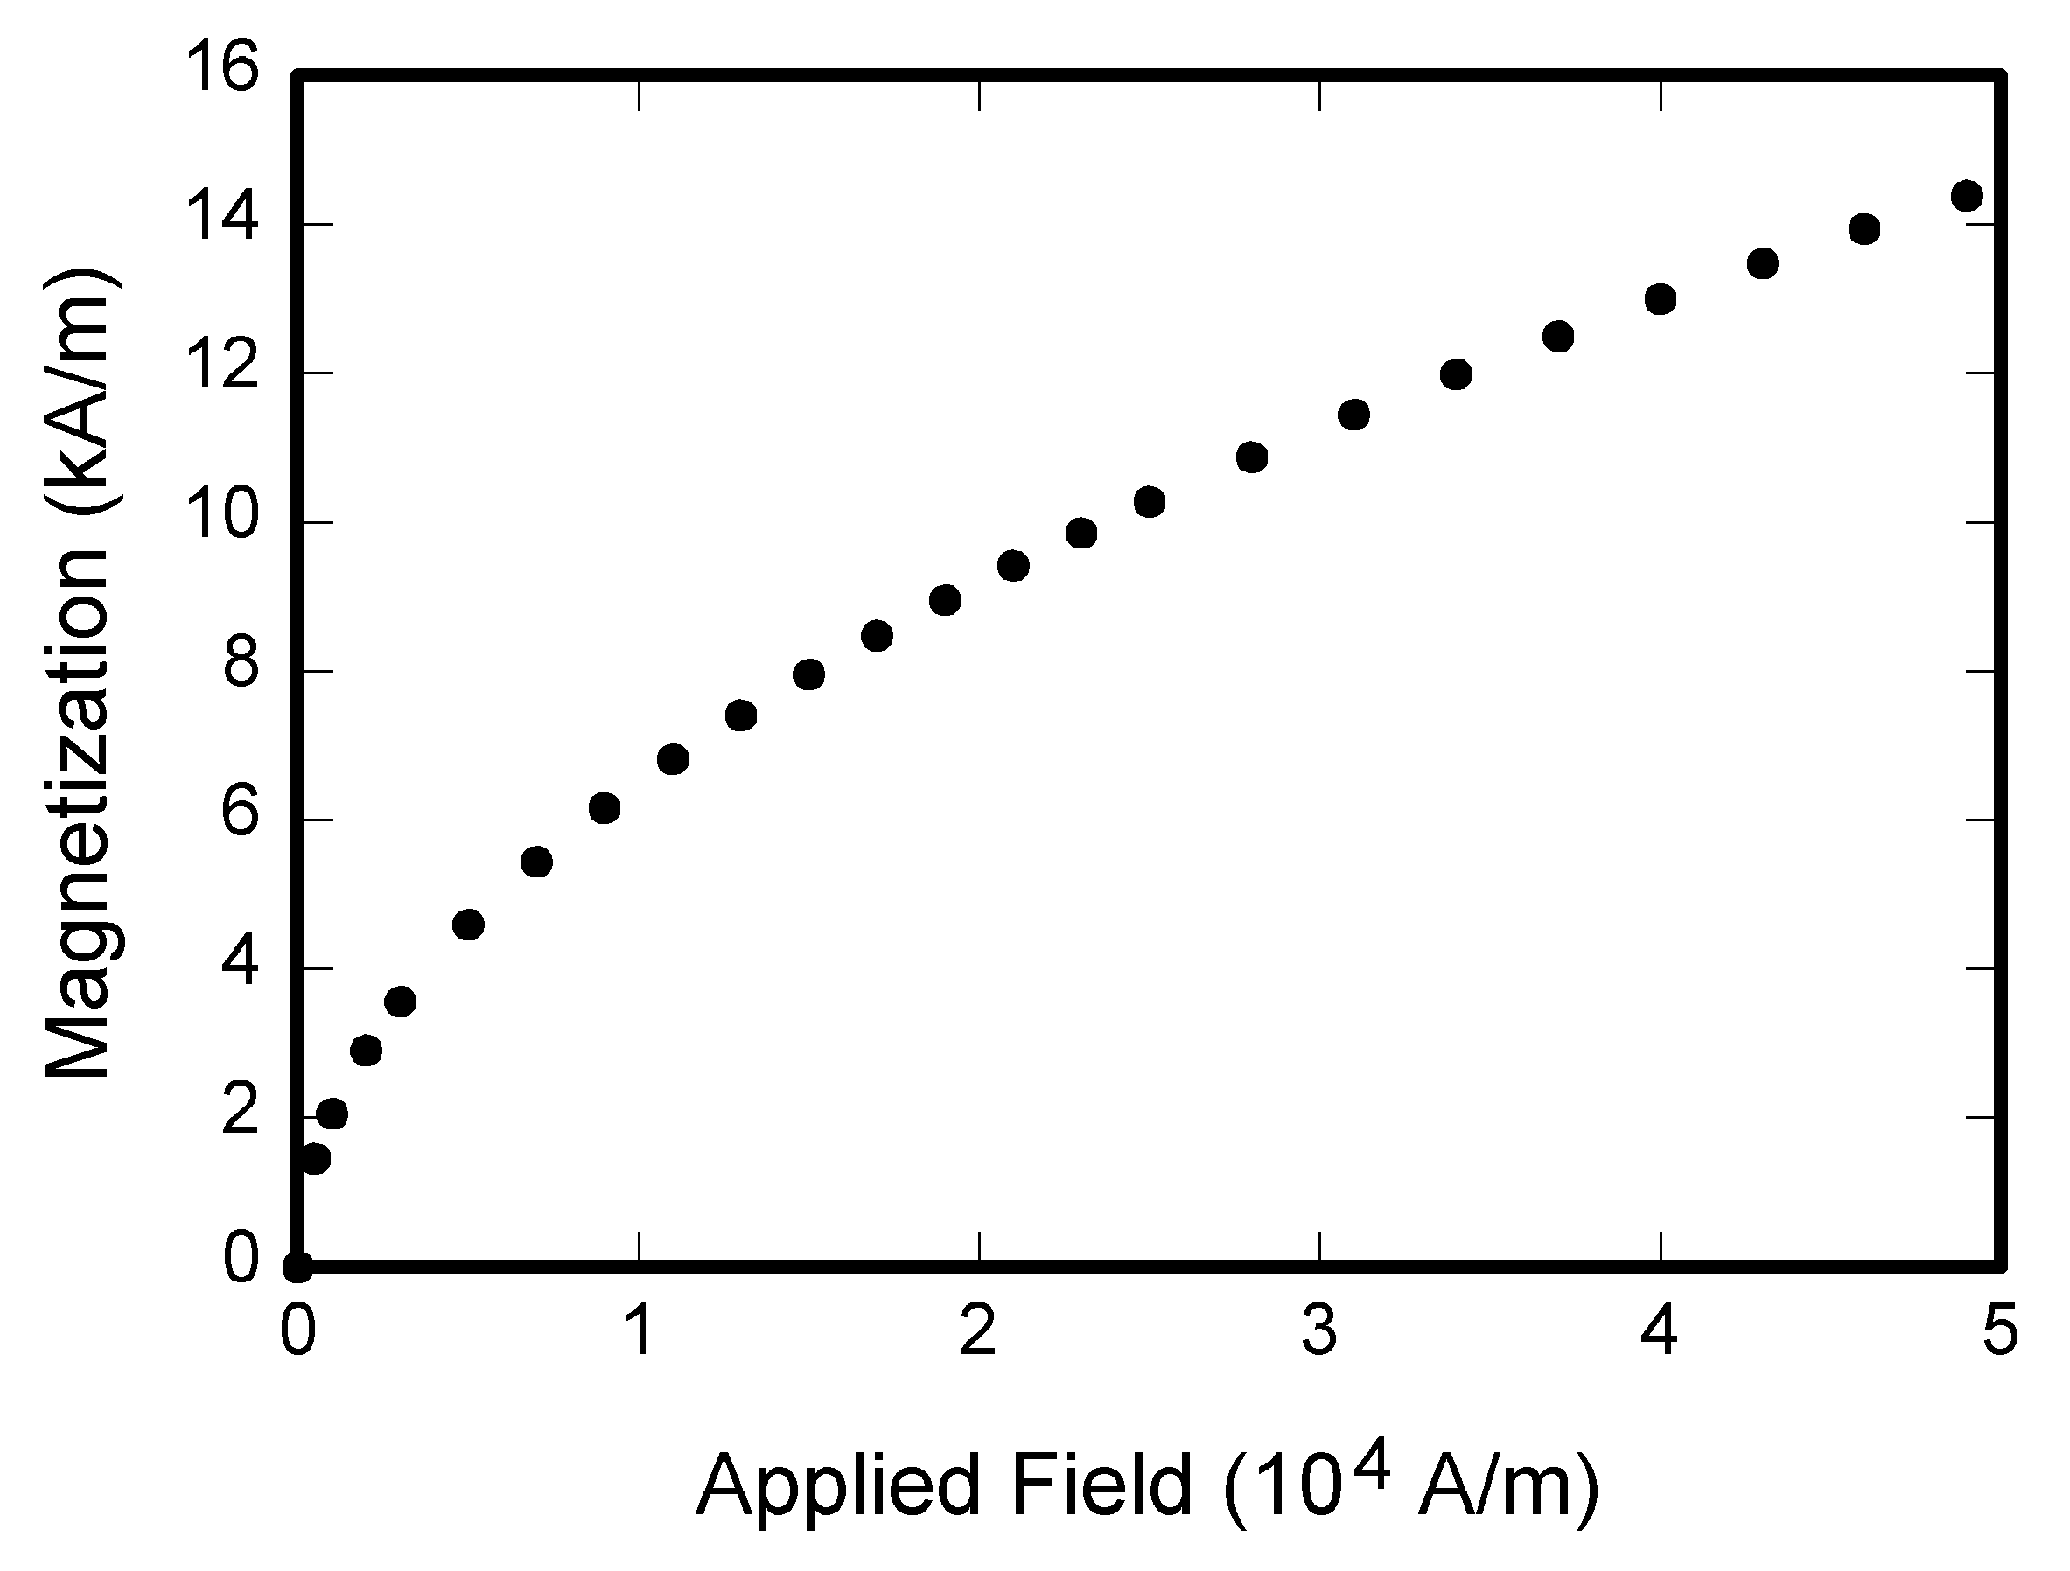
\includegraphics[width=\linewidth]{Photos/fig1.png}
        \caption{Caption 4}
        \label{fig:2d}
    \end{subfigure}

    \caption{2×2 grid of subfigures using subcaption.}
    \label{fig:grid_subcaption}
\end{figure}


% htbpH meaning
% h - here
% t - top
% b - bottom
% p - page
% H - try to place the figure here
% ! - Override most of LaTeX’s internal rules about float placement — it means “try harder to place it exactly where I ask.”
% htbp meaning - Try to place the figure here, otherwise at the top of the page, otherwise at the bottom, otherwise on a separate float page.

% figure - use for one column figure
% figure* - use for two column figure

% ##############################################